\begin{refsection}
\hypertarget{writing}{%
\chapter{Writing systems}\label{chap-writing}}

\section{Introduction}

Writing systems (or scripts) are collections of symbols and the rules for combining them in order to represent language. By some counts, there are now over 3,500 writing systems in the world. We will avoid the term \textit{letter} to refer to these symbols since they might represent not only individual sounds (see \chapref{chap-phonetics}, \textit{Phonetics}) but also syllables or even whole words. Therefore, the term \textit{character} is preferred.

\section{Pictographic and ideographic systems}

Etymologically, the terms \textit{pictographic} and \textit{ideographic} are compounds formed from \textit{picto-} (`picture'), \textit{ideo-} (`idea'), and \textit{grafos} (`writing'). In these systems, each character represents a word, an idea or a concept. Moreover, the characters are similar in appearance to the real-life representation of these concepts.

Although there are notable differences between the picto- and ideographic systems, these are not very relevant when it comes to linguistics problems. For this reason, we will combine these two types of script in a single category.

We often encounter these kinds of systems in contexts where there is a need to convey some idea that is not specific to a particular language. Many such symbols are widely used across cultures, such as the \textit{P} symbol used to represent a parking lot. A good example of a pictographic system is traffic and public signage (such as a crossed-out ice-cream cone to show that it is forbidden to eat food).

In linguistics problems these types of system are quite rare: usually, the relationship between the character and its meaning is so straightforward as to make the solution essentially effortless.

\section{Logographic systems}

In some ways, such scripts are highly similar to picto- and ideographic systems. The word \textit{logographic} is made up of two etymons: \textit{logos-} `word' and \textit{grafos-} `writing': in these systems, at least in principle, each character represents a word. In most cases, the logographic systems have their origin in picto- or ideographic systems, but the characters have evolved over time, thus losing their similarity with the real-life representation of the words they designate. For instance, many Chinese characters have developed from pictographic representations to logographic ones. Thus, the character for \texttr{sun}, which used to be represented as something like {\large{☉}}, is nowadays (in Modern Chinese) written as {\chinesetext{日}}. Similarly, the character for \texttr{moon/month}, initially represented as something like {\large{☽}}, has become {\chinesetext{月}} in Modern Chinese.

\section{Syllabic systems (syllabaries)}

Here, each character represents a syllable. Crucially, unlike some scripts that we will present below, each syllable is represented as a whole, without any clear relationship between characters denoting syllables that share some vowels or consonants.

One example of a syllabary is \textit{katakana}, one of the writing systems in use in Japan.

The following table gives some examples of katakana characters. Each character represents a syllable, consisting of a consonant and a vowel. Conventionally, these are written in a table in which the vowel spans across columns and the consonant across rows:

\begin{center}
    \begin{tabular}{|c|c|c|c|c|c|}
\hline
 & \cmubdata{a} & \cmubdata{i} & \cmubdata{u} & \cmubdata{e} & \cmubdata{o} \\ \hline
$\varnothing$ & {\jpn ア} & {\jpn イ} & {\jpn ウ} & {\jpn エ} & {\jpn オ} \\ \hline
\cmubdata{k}  & {\jpn カ} & {\jpn キ} & {\jpn ク} & {\jpn ケ} & {\jpn コ} \\ \hline
\cmubdata{s}  & {\jpn サ} & {\jpn シ} & {\jpn ス} & {\jpn セ} & {\jpn ソ} \\ \hline
\cmubdata{t}  & {\jpn タ} & {\jpn チ} & {\jpn ツ} & {\jpn テ} & {\jpn ト} \\ \hline
\end{tabular}
\end{center}

We can easily observe that the syllable is treated as a whole, and cannot be further divided into smaller components. For instance, the first line in the table corresponds to the absence of consonant (the character {\jpn ウ} represents the syllable \cmubdata{u}), but the other characters do not look anything like these symbols. Similarly, from knowing the characters for \cmubdata{ka} ({\jpn カ}), \cmubdata{ki} ({\jpn キ}), and \cmubdata{si} ({\jpn シ}) we cannot deduce the character for \cmubdata{sa} ({\jpn サ}).

\section{The Chinese writing system}

There are a lot of misconceptions about the Chinese writing system. It is erroneous to consider it either pictographic or ideographic: Chinese characters are not “pictures” representing meanings directly. Neither is it entirely logographic. In fact, it is a logo-syllabic system (a logo-syllabary). Some characters are indeed purely logographic (as we mentioned before), but they make up a very small percentage of the total number of characters. Most of the characters are formed by what we call the \textit{rebus principle}, where each character is formed by two components: a logographic part, approximately showing the meaning of that character (called the \textit{semantic} component) and a syllabic part, giving clues about the pronunciation of that character (called the \textit{phonetic} component).

For example, the character \cmubdata{ma\textsuperscript{3}} ({\chinesetext{马}}) is purely logographic and represents the word \texttr{horse}, while the character for \texttr{mother} ({\chinesetext{妈}}, \cmubdata{ma\textsuperscript{1}}) is logo-syllabic.\footnote{To transcribe Chinese words, we use a modified version of the \textit{pinyin} transcription system: the letters indicate the sounds and the digit indicates \OlympiadNewTerm{tone}, a distinctive property of the entire syllable that can distinguish meaning (see \sectref{sec:3.6}). In Chinese, syllables with different tones differ in the level and the trajectory of the voice's \OlympiadNewTerm{pitch}.} It is formed from the semantic component (cf. the logographic {\chinesetext{女}} \cmubdata{nü\textsuperscript{3}} \texttr{woman}) and the phonetic component {\chinesetext{马}}. Therefore, {\chinesetext{妈}} is a character whose meaning is related to \texttr{woman} and whose pronunciation is similar to that of {\chinesetext{马}}. Some more examples of logographic characters created by the rebus principle are:

\begin{center}
\begin{tabular}{@{} l@{~}c@{~}l  @{~}c@{~}l @{}}
{\chinesetext{机}} (\cmubdata{ji\textsuperscript{1}}, \texttr{machine}) & = & {\chinesetext{木}} (\cmubdata{mu\textsuperscript{4}}, \texttr{wood}) & + &  {\chinesetext{几}} (\cmubdata{ji\textsuperscript{3}}, \texttr{some})\\
{\chinesetext{唱}} (\cmubdata{chang\textsuperscript{4}}, \texttr{to sing}) & = & {\chinesetext{口}} (\cmubdata{kou\textsuperscript{3}}, \texttr{mouth}) & + & {\chinesetext{昌}} (\cmubdata{chang\textsuperscript{1}}, \texttr{prosperity})
\end{tabular}
\end{center}

\section{Alphabetic systems (alphabets)}
These are the most common systems in Europe and each character represents either a consonant or a vowel. In other words, each character represents a sound. Examples of these scripts are the Latin alphabet (used to write languages such as English, Romanian, Spanish, Italian, German, Polish, Turkish), the Greek alphabet (used for writing Greek), the Cyrillic alphabet (used to write some Slavic languages such as Russian, Ukrainian, Belarusian, Bulgarian, as well as many languages spoken in Russia), the Georgian alphabet (used for the Georgian language), and the Armenian alphabet (used for the Armenian language).

\section{Abjad systems}

In these systems, each character represents a consonant, while vowels are not written at all or shown as diacritics (i.e., small marks attached to the character). In broad terms, this type of system can be compared to syllabic systems, in the sense that each “complete”\ character represents a combination of a consonant and a vowel; but, unlike syllabaries, each component is represented separately, so the character can be broken down into subparts. \par

Some well-known abjads are used for Semitic languages, such as the Arabic and Hebrew scripts. Below we show some Arabic characters: \par
\begin{center}
    \begin{tabular}{|c|c|c|c|c|c|c|c|}
    \hline 
      & $\varnothing$ & \cmubdata{u} & \cmubdata{ū} & \cmubdata{a} & \cmubdata{ā} & \cmubdata{i} & \cmubdata{ī} \\ \hline
      $\varnothing$ \raisebox{1.2em}{\vphantom{a}} & \cellcolor[HTML]{808080} & \arbtext{\charstack{\char"25CC}{\hspace{-0.2em}\char"064F}}  &\arbtext{\char"0648\charstack{\char"25CC}{\hspace{-0.2em}\char"064F}}&\arbtext{\charstack{\char"25CC}{\hspace{-0.2em}\char"064E}}&\arbtext{\char"0627\charstack{\char"25CC}{\hspace{-0.2em}\char"064E}}&\arbtext{\charstack{\char"25CC}{\hspace{-0.2em}\raisebox{-0.1em}{\char"0650}}}& \arbtext{\char"064A\charstack{\char"25CC}{\hspace{-0.2em}\raisebox{-0.1em}{\char"0650}}}\\[0.5em] \hline 
      \cmubdata{b}\raisebox{1.2em}{\vphantom{a}} & \arbtext{ب} & \arbtext{بُ} & \arbtext{بُو} & \arbtext{بَ}& \arbtext{بَا}& \arbtext{بِ}& \arbtext{بِي}\\[0.5em] \hline
      \cmubdata{s}\raisebox{1.2em}{\vphantom{a}} & \arbtext{س} & \arbtext{سُ} & \arbtext{سُو} & \arbtext{سَ}& \arbtext{سَا}& \arbtext{سِ}& \arbtext{سِي}\\[0.5em] \hline
    \end{tabular}
\end{center}

The dotted circle is used to show the placement of the diacritics for \cmubdata{u}, \cmubdata{a}, and \cmubdata{i} relative to the consonant character: in Arabic, the same diacritic is used to mark both \cmubdata{a} and \cmubdata{i}, but in the former case it is placed above the consonant, and in the latter case it goes below the character marking the consonant.

\section{Abugida systems}

These systems are very similar to abjads, in the sense that each “complete”\ character represents a combination of a vowel and a consonant. However, in an abjad each character (without diacritics) represents a consonant and the diacritics, when used, append the corresponding vowels. In abugidas, a character without any diacritics or modifications represents a consonant followed by some vowel of the language (called the “default”\ or “inherent”\ vowel), and additional modifications are used to change that vowel to another one. Moreover, most abugidas will have some device to “delete”\ the vowel, so as to represent the consonant on its own.

Many languages of South and South-East Asia are written using abugidas. Here are some Burmese characters:

\begin{center}
    \begin{tabular}{|c|c|c|c|c|c|c|c|c|c|}
\hline
 & \cmubdata{a} & \cmubdata{aa} & \cmubdata{i} & \cmubdata{ii} & \cmubdata{u} & \cmubdata{uu} & \cmubdata{e} & \cmubdata{ai} & $\varnothing$ \\ \hline 
 $\varnothing$\vphantom{\Huge{A}} & \burmtext{\char"25CC} &\burmtext{ာ}&\burmtext{ိ}&\burmtext{ီ}&\burmtext{ု}&\burmtext{ူ}&\burmtext{ေ}&\burmtext{ဲ}& \burmtext{်} \\ [0.5em]\hline
\cmubdata{k}\vphantom{\Huge{A}} & \burmtext{က} & \burmtext{ကာ} & \burmtext{ကိ} & \burmtext{ကီ} & \burmtext{ကု} & \burmtext{ကူ} & \burmtext{ကေ} & \burmtext{ကဲ} & \burmtext{က်} \\ [0.5em] \hline
\cmubdata{s}\vphantom{\Huge{A}} & \burmtext{ဆ} & \burmtext{ဆာ} & \burmtext{ဆိ} & \burmtext{ဆီ} & \burmtext{ဆု} & \burmtext{ဆူ} & \burmtext{ဆေ} & \burmtext{ဆဲ} & \burmtext{ဆ်} \\ [0.5em] \hline
\end{tabular}
\end{center}

We can observe that the default vowel is \cmubdata{a} (representing the basic form of each consonant). Adding a loop will change the vowel from \cmubdata{a} to \cmubdata{aa} (long \cmubdata{a}) while adding an L-like symbol below changes the vowel from \cmubdata{a} to \cmubdata{u}, etc.

A very interesting abugida system is Cree Syllabics, used to write aboriginal languages of Canada. In this system, the vowel change is not shown by diacritics, but rather by rotating the character (by 90$^{\circ}$, 180$^{\circ}$ or 270$^{\circ}$) or by mirroring it, depending on its shape. Below we show a table with some Cree characters.

\begin{center}
    \begin{tabular}{ccccccccccc}
\multicolumn{5}{c}{{Rotation}} & \hphantom{Indent}  & \multicolumn{5}{c}{{Mirroring}} \\ \cline{1-5} \cline{7-11} 
\multicolumn{1}{|c|}{} & \multicolumn{1}{c|}{\cmubdata{a}} & \multicolumn{1}{c|}{\cmubdata{e}} & \multicolumn{1}{c|}{\cmubdata{i}} & \multicolumn{1}{c|}{\cmubdata{o}} & \multicolumn{1}{c|}{} & \multicolumn{1}{c|}{} & \multicolumn{1}{c|}{\cmubdata{a}} & \multicolumn{1}{c|}{\cmubdata{e}} & \multicolumn{1}{c|}{\cmubdata{i}} & \multicolumn{1}{c|}{\cmubdata{o}} \\ \cline{1-5} \cline{7-11} 
\multicolumn{1}{|c|}{$\varnothing$\vphantom{\huge{A}}} & \multicolumn{1}{c|}{\creetext{ᐊ}} & \multicolumn{1}{c|}{\creetext{ᐁ}} & \multicolumn{1}{c|}{\creetext{ᐃ}} & \multicolumn{1}{c|}{\creetext{ᐅ}} & \multicolumn{1}{c|}{} & \multicolumn{1}{c|}{\cmubdata{k}} & \multicolumn{1}{c|}{\creetext{ᑲ}} & \multicolumn{1}{c|}{\creetext{ᑫ}} & \multicolumn{1}{c|}{\creetext{ᑭ}} & \multicolumn{1}{c|}{\creetext{ᑯ}} \\ \cline{1-5} \cline{7-11} 
\multicolumn{1}{|c|}{\cmubdata{p}\vphantom{\huge{A}}} & \multicolumn{1}{c|}{\creetext{ᐸ}} & \multicolumn{1}{c|}{\creetext{ᐯ}} & \multicolumn{1}{c|}{\creetext{ᐱ}} & \multicolumn{1}{c|}{\creetext{ᐳ}} & \multicolumn{1}{c|}{} & \multicolumn{1}{c|}{\cmubdata{m}} & \multicolumn{1}{c|}{\creetext{ᒪ}} & \multicolumn{1}{c|}{\creetext{ᒣ}} & \multicolumn{1}{c|}{\creetext{ᒥ}} & \multicolumn{1}{c|}{\creetext{ᒧ}} \\ \cline{1-5} \cline{7-11} 
\multicolumn{1}{|c|}{\cmubdata{t}\vphantom{\huge{A}}} & \multicolumn{1}{c|}{\creetext{ᑕ}} & \multicolumn{1}{c|}{\creetext{ᑌ}} & \multicolumn{1}{c|}{\creetext{ᑎ}} & \multicolumn{1}{c|}{\creetext{ᑐ}} & \multicolumn{1}{c|}{} & \multicolumn{1}{c|}{\cmubdata{n}} & \multicolumn{1}{c|}{\creetext{ᓇ}} & \multicolumn{1}{c|}{\creetext{ᓀ}} & \multicolumn{1}{c|}{\creetext{ᓂ}} & \multicolumn{1}{c|}{\creetext{ᓄ}} \\ \cline{1-5} \cline{7-11} 
\end{tabular}
\end{center}

We can observe, conceptually, that the preference is for mirroring (right-hand table) since sometimes the same shape is used for two different consonants (\cmubdata{k} \creetext{ᑲ}, vertically, and \cmubdata{n} \creetext{ᓇ}, horizontally). The characters obtained by rotation are used only where mirroring is not possible due to symmetry reasons (a mirrored \creetext{ᐁ} is still \creetext{ᐁ}). Therefore, we can deduce that if a character cannot be mirrored (it has a symmetry axis), the vowel change will be represented by a clockwise 90$^\circ$ rotation (vowels change in the sequence \cmubdata{a \rightarrow\ i \rightarrow\ o \rightarrow\ e \rightarrow\ a}). The change of vowel by mirroring is performed either vertically (\cmubdata{a \Leftrightarrow\ o} and \cmubdata{e \Leftrightarrow\ i}), or horizontally (\cmubdata{a~\Leftrightarrow~i} and \cmubdata{e~\Leftrightarrow~o}). The rotation and mirroring patterns of the Cree characters are shown below.

\begin{center}
    \begin{tabular}{ccccP{1.5em}:P{1.5em}}
\multicolumn{3}{c}{{Rotation}} & \hphantom{Indent} & \multicolumn{2}{c}{{Mirroring}} \\
 & \creetext{ᐁ} &  &  & \creetext{ᑲ} & \creetext{ᑯ} \\ \cdashline{5-6}
\creetext{ᐅ} & \Large{$\circlearrowright$} & \creetext{ᐊ} &  & \creetext{ᑭ} & \creetext{ᑫ} \\
 & \creetext{ᐃ} &  \multicolumn{4}{c}{} 
\end{tabular}
\end{center}

\section{Featural systems}

This is the last type of writing system and probably the least common. In this system, each character highlights the phonetic or phonological features of the sounds it designates. For example, in the Korean writing system (\textit{hangul}), the characters corresponding to the sounds \cmubdata{p}, \cmubdata{p*}, \cmubdata{p\textsuperscript{h}}, and \cmubdata{m} ({\koreantext{ㅂ}}, {\koreantext{ㅃ}}, {\koreantext{ㅍ}}, {\koreantext{ㅁ}}, respectively) are highly similar: all of them derive from a square. This is because all these sounds are bilabial (as we will see in the next chapter). When pronouncing them we use our lips (see the next chapter for more details on how to describe different sounds) and the square is meant to evoke the mouth seen from the front.

The property of being featural cuts across the other criteria we have used: the main characteristic of these systems is the fact that the properties of symbols are based on features of the sounds they represent, not the nature of the mapping between character and sound. For instance, the hangul writing system marks each character, whether vowel or consonant, individually, so it can also be considered an alphabet.

\begin{problem}{\langnameHmong}{\nameIDerzhanski}{\LOYear{\MSKAbbr}{2003}}

Here are several words and phrases in the Hmong Daw language written in Shong Lue Yang's script and the missionaries' alphabet, as well as their English translations:

{\centering\begin{longtable}{rccc}
    \hmongline{\char"16B09\ \charstack{\char"16B11}{\char"16B32}\char"16B1D\ \charstack{\char"16B0B}{\char"16B30}\char"16B2C}{kev ntsuas no}{degree}
    \hmongline{\char"16B05\char"16B1F}{hauv}{inside}
    \hmongline{\charstack{\char"16B05}{\char"16B36}\char"16B21\ \charstack{\char"16B0F}{\char"16B32}\char"16B21\ \charstack{\char"16B0B}{\char"16B30}\char"16B2F}{raug raws cai}{legal}
    \hmongline{\char"16B0D\char"16B25\ \charstack{\char"16B07}{\char"16B32}\char"16B26}{hloov mus}{transfer}
    \hmongline{\charstack{\char"16B11}{\char"16B30}\char"16B23}{qhua}{guest}
    \hmongline{\charstack{\char"16B13}{\char"16B36}\char"16B24\ \charstack{\char"16B13}{\char"16B32}\char"16B1E\ \charstack{\char"16B17}{\char"16B36}\char"16B2C}{yog los nag}{it is raining}
    \hmongline{\char"16B19\ \charstack{\char"16B16}{\char"16B32}\char"16B24}{kwv yees}{guess}
    \hmongline{\charstack{\char"16B03}{\char"16B32}\char"16B21\ \charstack{\char"16B09}{\char"16B36}\char"16B2F\ \char"16B07\char"16B1E}{ris ceg luv}{Bermuda shorts}
    \hmongline{\charstack{\char"16B0D}{\char"16B36}\char"16B2C}{\pbblank}{bird}
    \hmongline{\charstack{\char"16B19}{\char"16B30}\char"16B2F}{\pbblank}{lobster}
    \hmongline{\charstack{\char"16B0B}{\char"16B32}\char"16B1F\ \charstack{\char"16B07}{\char"16B32}\char"16B1E}{\pbblank}{speak}
    \hmongline{\char"16B13\char"16B23\ \charstack{\char"16B11}{\char"16B36}\char"16B26\ \char"16B03}{\pbblank}{dizzy}
    \hmongline{\pbblank}{hluav}{ash}
    \hmongline{\pbblank}{li cas}{how?}
    \hmongline{\pbblank}{neeg ntse}{smart, wise}
    \hmongline{\pbblank}{yawg}{grandfather}
\end{longtable}}

\begin{assgts}
\item \fillblanks
\end{assgts}

\begin{tblsWarning}
In the missionaries' alphabet, the letter \cmubdata{w} represents a specific vowel. The letters \cmubdata{g}, \cmubdata{s}, \cmubdata{v} at the ends of the syllables are not consonants; instead, they denote tones (specific ways of pronouncing the vowels).
\end{tblsWarning}
\end{problem}

\begin{mysolution}
First thing we need to notice is that we do not have to provide English translations. This is one of the main characteristics of writing system problems. Moreover, the fact that we are not asked to provide English translations means that the translations are probably not relevant to solving the problem.

\note{This is not always true; it is just a rule of thumb. It is possible for some problems that, although no translations are required, they can still be relevant – for example, based on semantic considerations.}

We also need to keep in mind that for writing-systems problems the writing direction is relevant (from left to right or from right to left). Moreover, we notice that in Hmong the characters are grouped in clusters of one or two, while in the Latin transcription, they are grouped in syllables. Therefore, we can deduce that each group of characters represents a syllable.

We can begin by noticing the diacritics placed above some syllables. Since the mark \hmongtext{\charstack{{\char"25CC}}{\char"16B36}} appears the greatest number of times, we can begin with it and observe that it is transliterated by the letter \cmubdata{g} at the end of the syllable. Moreover, reading the footnote, we find out that this letter does not represent a consonant or a vowel per se, but rather the syllable tone. Finally, based on example 3, in which the syllable containing the \cmubdata{g} tone appears first, we deduce that the writing direction for syllables is from left to right.

Using a similar reasoning, we identify the four possible tone marks: $\varnothing$ (\hmongtext{\charstack{{\char"25CC}}{\char"16B30}}), \cmubdata{g} (\hmongtext{\charstack{{\char"25CC}}{\char"16B36}}), \cmubdata{s} (\hmongtext{\charstack{{\char"25CC}}{\char"16B32}}), \cmubdata{v} (\hmongtext{{\char"25CC}}). It is important to notice that the lack of a diacritic mark in Hmong is not equivalent to the lack of tone in the Latin transcription. If there is no diacritic above the syllable in Hmong, the Latin correspondent is the tone \cmubdata{v}, while if there is no tone marking in the Latin transcription (the syllable ends in a vowel and not in \cmubdata{g}, \cmubdata{s}, or \cmubdata{v}), then the Hmong syllable will have a dot on top of the syllable. Therefore, we can consider the tone marking, to some extent, as an abugida system, in which the default tone is \cmubdata{v} and the change in tone or the lack thereof is marked by diacritics.

We are left to find out how the syllable is formed, i.e., which character represents the consonant and which character represents the vowel. Comparing examples 2 and 3, we notice that the first character of the first syllable is identical (except for the tone, which we already identified) and the two syllables (\cmubdata{hauv}, \cmubdata{raug}) have the same vowel (or sequence of vowels); thus the first symbol represents the vowel and the second one the consonant.

Another indication towards this order between the vowel and the consonant is that the tones, which are described as “specific ways of pronouncing the vowels”, are generally marked above the first character, suggesting that the first character indeed refers to the vowel.

Based on this information, we can easily identify all the characters in this script. An important observation is the way the consonant \cmubdata{k} is marked. Based on examples 1 and 7, we notice that this consonant is not written, but rather treated as a default consonant. As a result, if in the Hmong script no consonant is written, we understand that the consonant is \cmubdata{k}. This is a particularly interesting writing system which cannot be easily fitted into any of the aforementioned categories of scripts, having characteristics of different types. On the one hand, we can consider it an alphabet since each consonant (consonant cluster) and vowel (or sequence of vowels) have individual characters (however, there are no characters for vowel-consonant combinations). On the other hand, the consonant \cmubdata{k} is not written, so it can be considered a default consonant and all the other symbols are used to change this consonant to another one (resulting in an abugida-like system in which there is a default consonant, rather than a vowel), just as in the case of tones (in which the abugida characteristics are much more obvious, having a default tone and a diacritic to remove it).

Based on all of the above, we can write the solution and solve the tasks.

\begin{solutions}[label=Solution 2.1\alph*]
\item
    \begin{multicols}{2}
    \begin{enumerate}[label = (\arabic*)]
        \item \cmubdata{noog}
        \item \cmubdata{cw}
        \item \cmubdata{hais lus}
        \item \cmubdata{qhov muag kiv}
        \item \hmongtext{\char"16B11\char"16B25}
        \item \hmongtext{\charstack{\char"16B03}{\char"16B30}\char"16B1E\ \charstack{\char"16B17}{\char"16B32}\char"16B2F}
        \item \hmongtext{\charstack{\char"16B16}{\char"16B36}\char"16B2C\ \charstack{\char"16B09}{\char"16B30}\char"16B1D}
        \item \hmongtext{\charstack{\char"16B0F}{\char"16B36}\char"16B24}
    \end{enumerate}
    \end{multicols}
\end{solutions}

\rules
\begin{itemize}
    \item Syllables are written from left to right.
    \item Syllable structure: $\stackrel{3}{1} \stackrel{~}{2}$
    \item 1 = vowel / vowel cluster (syllable nucleus) -- \cmubdata{a} (\hmongtext{\char"16B17}), \cmubdata{e} (\hmongtext{\char"16B09}), \cmubdata{i} (\hmongtext{\char"16B03}), \cmubdata{o} (\hmongtext{\char"16B13}), \cmubdata{u} (\hmongtext{\char"16B07}), \cmubdata{w} (\hmongtext{\char"16B19}), \cmubdata{ai} (\hmongtext{\char"16B0B}), \cmubdata{au} (\hmongtext{\char"16B05}), \cmubdata{aw} (\hmongtext{\char"16B0F}), \cmubdata{ee} (\hmongtext{\char"16B16}), \cmubdata{oo} (\hmongtext{\char"16B0D}), \cmubdata{ua} (\hmongtext{\char"16B11})
    \item 2 = consonant (beginning of the syllable, onset) -- \cmubdata{c} (\hmongtext{\char"16B2F}), \cmubdata{h} (\hmongtext{\char"16B1F}), \cmubdata{k} ($\varnothing$), \cmubdata{l} (\hmongtext{\char"16B1E}), \cmubdata{m} (\hmongtext{\char"16B26}), \cmubdata{n} (\hmongtext{\char"16B2C}), \cmubdata{r} (\hmongtext{\char"16B21}), \cmubdata{y} (\hmongtext{\char"16B24}), \cmubdata{hl} (\hmongtext{\char"16B25}), \cmubdata{nts} (\hmongtext{\char"16B1D}), \cmubdata{qh} (\hmongtext{\char"16B23})
    \item 3 = tone -- $\varnothing$ (\hmongtext{\charstack{\LARGE{\char"25CC}}{\char"16B30}}), \cmubdata{g} (\hmongtext{\charstack{\LARGE{\char"25CC}}{\char"16B36}}), \cmubdata{s} (\hmongtext{\charstack{\LARGE{\char"25CC}}{\char"16B32}}), \cmubdata{v} (\hmongtext{\LARGE{\char"25CC}})
\end{itemize}
\end{mysolution}

\begin{problem}{\langnameLuwian}{\nameAZhurinsky}{\LOYear{\MSKAbbr}{1979}}
The following are some inscriptions in the Luwian language. They correspond to some names of regions: \cmubdata{Khamatu}, \cmubdata{Palaa}, names of cities: \cmubdata{Kurkuma}, \cmubdata{Tuvanava} and names of kings: \cmubdata{Varpalava}, \cmubdata{Tarkumuva}.
\begin{center}
    \begin{tabular}{rc@{\hskip0.5in}rc}
         1.& \luwtext{\char"145EC{\hspace{-0.15em}\large{\char"145B1}}\char"14578\char"144CA\char"145EC\char"14411} &
         4.& \luwtext{\char"14578\char"144CA\char"14413\char"14506}  \\[0.3em]
         2.&\luwtext{\char"145DC{\hspace{-0.15em}\large{\char"145B1}}\char"145DC\char"14485\char"14502} &
         5.& \luwtext{\char"1445B{\hspace{-0.05em}\large{\char"145B1}}\char"145DC\char"1447F\char"145EC\char"14411}  \\[0.3em]
         3.& \luwtext{\char"14462\char"145EC\char"14424\char"145EC\char"14502} &
         6.& \luwtext{\char"144EF\char"14485\char"14462\char"14506}  \\[0.3em]
    \end{tabular}
\end{center}
\begin{assgts}
\item \detcorr
\item \taskWriteIn{\langnameLuwian}:
\begin{multicols}{3}
\begin{enumerate}[start = 7]
    \item \cmubdata{king Parta}
    \item \cmubdata{king Artur}
    \item \cmubdata{city Tartu}
    \item \cmubdata{region Tuva}
    \item \cmubdata{city Narva}
    \blankitem
\end{enumerate}
\end{multicols}
\end{assgts}
\end{problem}

\begin{mysolution}
According to the introduction, the six inscriptions correspond to three categories of words: names of kings, cities, and regions. Moreover, we notice that the last character of each inscription does not appear anywhere else inside the inscription. Therefore, we can assume that these characters denote the idea of \texttr{king}, \texttr{city}, and \texttr{region}; thus we can divide the six inscriptions into three categories based on the last character:

\begin{center}
    \begin{tabular}{|c|c|c|}
    \hline
    I & II & III \\\hline
     \luwtext{\char"145EC{\hspace{-0.15em}\large{\char"145B1}}\char"14578\char"144CA\char"145EC\char"14411}& \luwtext{\char"145DC{\hspace{-0.15em}\large{\char"145B1}}\char"145DC\char"14485\char"14502}&\luwtext{\char"144EF\char"14485\char"14462\char"14506} \\
     \luwtext{\char"1445B{\hspace{-0.05em}\large{\char"145B1}}\char"145DC\char"1447F\char"145EC\char"14411}& \luwtext{\char"14462\char"145EC\char"14424\char"145EC\char"14502}&\luwtext{\char"14578\char"144CA\char"14413\char"14506} \\ \hline
    \end{tabular}
\end{center}

We can safely assume that this writing system is not alphabetic since each inscription has four or five characters, while their transcriptions have between five and nine characters. Moreover, it is unlikely that this system is an abugida or an abjad since there do not seem to be any diacritics appended (or similar characters). Therefore, it is most likely a syllabic system. To check this, we can try to divide the words in Latin transcription into syllables to check if the number of characters matches the number of syllables. (If you are unsure how to do this, see the discussion in \chapref{chap-phonetics}.)

\cmubdata{Kha-ma-tu} and \cmubdata{Pa-la-a} each have three syllables. Therefore, we know for sure they correspond to group III (because it is the only group in which both inscriptions have four syllables – three for the actual name and one to show the category).

\cmubdata{Kur-ku-ma} and \cmubdata{Tu-va-na-va} have three and four syllables and the only category that matches it is II, so we deduce that this corresponds to the cities. Moreover, since the number of syllables is different, we can already make the correct correspondences: 2 -- \cmubdata{Kurkuma} and 3 -- \cmubdata{Tuvanava}.

The last group is that for kings and both words have indeed four syllables (\cmubdata{Var-pa-la-va} and \cmubdata{Tar-ku-mu-va}). We get:

\begin{center}
    \begin{tabular}{|c|c|c|}
    \hline
    Kings & Cities & Regions \\\hline
     \luwtext{\char"145EC{\hspace{-0.15em}\large{\char"145B1}}\char"14578\char"144CA\char"145EC\char"14411}& \luwtext{\char"145DC{\hspace{-0.15em}\large{\char"145B1}}\char"145DC\char"14485\char"14502}&\luwtext{\char"144EF\char"14485\char"14462\char"14506} \\
     & \cmubdata{Kurkuma} & \\ \hline
     \luwtext{\char"1445B{\hspace{-0.05em}\large{\char"145B1}}\char"145DC\char"1447F\char"145EC\char"14411}& \luwtext{\char"14462\char"145EC\char"14424\char"145EC\char"14502}&\luwtext{\char"14578\char"144CA\char"14413\char"14506} \\
     & \cmubdata{Tuvanava} & \\\hline
    \end{tabular}
\end{center}

Looking at the script representation of \cmubdata{Kurkuma}, we notice that the first two characters are very similar and they only differ by a little line placed on the bottom-right. Therefore, most likely, those two characters represent the syllables \cmubdata{kur} and \cmubdata{ku} and the little line on the bottom-right marks the consonant \cmubdata{r} at the end of the syllable. This is also confirmed by the fact that the names of the two kings both start with a syllable ending in \cmubdata{r} (\cmubdata{Va\textbf{r}-pa-la-va} and \cmubdata{Ta\textbf{r}-ku-mu-va}) and in both cases the first character has that line on the bottom right. Therefore, we deduce that the syllables are written from left to right and at the end we write the character showing the category they belong to (regions, cities or kings).

The rest of the correspondences are easily determined: the first character of \cmubdata{Tuvarnava} corresponds to the syllable \cmubdata{tu} and this syllable is also found in one of the regions' names (third character). The only region that contains the syllable \cmubdata{tu} is \cmubdata{Khamatu}, thus 6 -- \cmubdata{Khamatu} and 4 -- \cmubdata{Palaa}.

Among the two kings' names, one begins with \cmubdata{var} (which we already know from the city \cmubdata{Tu-\textbf{va}-na-\textbf{va}}, adding the line representing final \cmubdata{r}), so we get the correspondences 1 -- \cmubdata{Varpalava} and 5 -- \cmubdata{Tarkumuva}.

Now we have all the information needed to solve the tasks.

\begin{solutions}
    \item \begin{enumerate}

    \begin{multicols}{3}
        \item king \cmubdata{Varpalava}
        \item city  \cmubdata{Kurkuma}
        \item city  \cmubdata{Tuvanava}
        \item region  \cmubdata{Palaa}
        \item king \cmubdata{Tarkumuva}
        \item region  \cmubdata{Khamatu}
    \end{multicols}
    \end{enumerate}
    \item \begin{enumerate}[start = 7]

    \begin{multicols}{3}
        \item \luwtext{\char"14578{\hspace{-0.05em}\large{\char"145B1}}\char"1445B\char"14411}
        \item \luwtext{\char"14413{\hspace{-0.1em}\large{\char"145B1}}\char"14462{\hspace{0em}\large{\char"145B1}}\char"14411}
        \item \luwtext{\char"1445B{\hspace{-0.05em}\large{\char"145B1}}\char"14462\char"14502}
        \item \luwtext{\char"14462\char"145EC\char"14506}
        \item \luwtext{\char"14424{\hspace{0em}\large{\char"145B1}}\char"145EC\char"14502}
        \item[] \vphantom{\luwtext{\char"14424{\hspace{0em}\large{\char"145B1}}\char"145EC\char"14502}}
    \end{multicols}
    \end{enumerate}
\end{solutions}

\rules

Syllabic system, left-to-right. In the end, there is a character showing the category to which the names belong: 
\begin{center}
\hfill\luwtext{\char"14411} for kings,
\hfill\luwtext{\char"14502} for cities, and 
\hfill\luwtext{\char"14506} for regions.\hfill\hbox{}
\end{center}

Each character represents a combination of a consonant and a vowel and adding a line on the bottom-right ({\hmongtext{\LARGE{\char"25CC}}}\luwtext{{\hspace{-0.05em}\large{\char"145B1}}}) marks the addition of the consonant \cmubdata{r} at the end of the syllable:

\begin{center}
    \begin{tabular}{|c|c|c|cccc}
\cline{1-3} \cline{5-7}
 & \cmubdata{a} & \cmubdata{u} & \multicolumn{1}{c|}{\hphantom{Indent}} & \multicolumn{1}{c|}{} & \multicolumn{1}{c|}{\cmubdata{a}} & \multicolumn{1}{c|}{\cmubdata{u}} \\ \cline{1-3} \cline{5-7}
$\varnothing$ & \luwtext{\char"14413} &  & \multicolumn{1}{c|}{} & \multicolumn{1}{c|}{\cmubdata{n}} & \multicolumn{1}{c|}{\luwtext{\char"14424}} & \multicolumn{1}{c|}{} \\ \cline{1-3} \cline{5-7}
\cmubdata{k} &  & \luwtext{\char"145DC} & \multicolumn{1}{c|}{} & \multicolumn{1}{c|}{\cmubdata{p}} & \multicolumn{1}{c|}{\luwtext{\char"14578}} & \multicolumn{1}{c|}{} \\ \cline{1-3} \cline{5-7}
\cmubdata{kh} & \luwtext{\char"144EF} &  & \multicolumn{1}{c|}{} & \multicolumn{1}{c|}{\cmubdata{t}} & \multicolumn{1}{c|}{\luwtext{\char"1445B}} & \multicolumn{1}{c|}{\luwtext{\char"14462}} \\ \cline{1-3} \cline{5-7}
\cmubdata{l} & \luwtext{\char"144CA} &  & \multicolumn{1}{c|}{} & \multicolumn{1}{c|}{\cmubdata{v}} & \multicolumn{1}{c|}{\luwtext{\char"145EC}} & \multicolumn{1}{c|}{} \\ \cline{1-3} \cline{5-7}
\cmubdata{m} & \luwtext{\char"14485} & \luwtext{\char"1447F} &  &  &  &  \\ \cline{1-3}
\end{tabular}
\end{center}
\end{mysolution}

\begin{discussion}

This is a syllabic type of system since each character represents a syllable. The only exception is the final character which is logographic (maybe even pictographic, considering that the symbol for `region' is composed of two symbols for `city', reflecting that a region is made up of more cities).

A possible issue when solving the problem is the syllabification of the word \cmubdata{Palaa}. Normally, we would have been tempted to syllabify it as \cmubdata{Pa-laa}, assuming the \cmubdata{aa} represents a long vowel (similar to problem 2.1). Nevertheless, if we had done that, the region Palaa would have had only three characters (two characters for the syllables \cmubdata{pa} and \cmubdata{laa} and one logographic character for region). Since we do not have any three-character inscriptions, we chose to syllabify the word as \cmubdata{Pa-la-a}.
\end{discussion}

\begin{problem}{\langnameTagbanwa}{\nameVNeacsu}{\LOYear{\JOLAbbr}{2022}}
Here are some words related to the mythology of the Tagbanwa people, written in the traditional script. They represent deities (\cmubdata{Mangindusa}, \cmubdata{Bugwasin}, \cmubdata{Tungkuyanin}, \cmubdata{Tumangkuyun}), names of spirits (\cmubdata{Kiyabusan}), rituals and words related to rituals (\cmubdata{Kapupusan}, \cmubdata{kadiyang}), as well as mythical places (\cmubdata{Balugu}).  Their Latin transcriptions are given \OlympiadRandomOrder{}:\footnote{\textit{Note}: Due to the contest taking place online, a slightly different format of the problem was used.}
\vskip\baselineskip
\begin{center}
    \begin{tabular}{|c|c|c|c|c|c|c|c|}
    \hline
    1.&2.&3.&4.&5.&6.&7.&8.\\ \hline
    \begin{tabular}{@{}c@{}}
        \\
         \tagbwtext{\char"1770} \\ [0.3em]
         \tagbwtext{\char"1767\hspace{-0.1em}\char"1773} \\ [0.3em]
         \tagbwtext{\char"1765\hspace{-0.1em}\char"1772} \\ [0.3em]
         \tagbwtext{\char"176B}\\\\
    \end{tabular}
    & \begin{tabular}{@{}c@{}}
        \\
         \tagbwtext{\char"1770\hspace{-0.1em}\char"1772} \\ [0.3em]
         \tagbwtext{\char"176F} \\ [0.3em]
         \tagbwtext{\char"1764} \\ [0.3em]
         \tagbwtext{\char"176A\hspace{-0.1em}\char"1773}\\\\
    \end{tabular}
    &\begin{tabular}{@{}c@{}}
        \\
         \tagbwtext{\char"1768\hspace{-0.1em}\char"1772} \\ [0.3em]
         \tagbwtext{\char"176C} \\ [0.3em]
         \tagbwtext{\char"1763\hspace{-0.1em}\char"1773} \\ [0.3em]
         \tagbwtext{\char"1766\hspace{-0.1em}\char"1773}\\\\
    \end{tabular}
    &\begin{tabular}{@{}c@{}}
        \\
         \tagbwtext{\char"176C\hspace{-0.1em}\char"1773} \\ [0.3em]
         \tagbwtext{\char"1763\hspace{-0.1em}\char"1773} \\ [0.3em]
         \tagbwtext{\char"176B} \\ [0.3em]
         \tagbwtext{\char"1766\hspace{-0.1em}\char"1773}\\\\
    \end{tabular}
    &\begin{tabular}{@{}c@{}}
        \\
         \tagbwtext{\char"1770} \\ [0.3em]
         \tagbwtext{\char"176A\hspace{-0.1em}\char"1773} \\ [0.3em]
         \tagbwtext{\char"176C\hspace{-0.1em}\char"1773} \\ [0.3em]
         \tagbwtext{\char"1763\hspace{-0.1em}\char"1772}\\\\
    \end{tabular}
    & \begin{tabular}{@{}c@{}}
        \\
         \tagbwtext{\char"1764\hspace{-0.1em}\char"1773} \\ [0.3em]
         \tagbwtext{\char"176E\hspace{-0.1em}\char"1773} \\ [0.3em]
         \tagbwtext{\char"176A}\\\\
    \end{tabular}
    &\begin{tabular}{@{}c@{}}
        \\
         \tagbwtext{\char"176C} \\ [0.3em]
         \tagbwtext{\char"1767\hspace{-0.25em}\char"1772} \\ [0.3em]
         \tagbwtext{\char"1763}\\\\
    \end{tabular}
    &\begin{tabular}{@{}c@{}}
        \\
         \tagbwtext{\char"1770} \\ [0.3em]
         \tagbwtext{\char"1769\hspace{-0.1em}\char"1773} \\ [0.3em]
         \tagbwtext{\char"1769\hspace{-0.1em}\char"1773} \\ [0.3em]
         \tagbwtext{\char"1763}\\\\
    \end{tabular}
     \\ \hline 
    \end{tabular}
\end{center}

\begin{enumerate}[label = \Alph*.]

\begin{multicols}{4}
    \item \cmubdata{balugu}
    \item \cmubdata{bugawasin}
    \item \cmubdata{kadiyang}
    \item \cmubdata{kapupusan}
    \item \cmubdata{kiyabusan}
    \item \cmubdata{mangindusa}
    \item \cmubdata{tumangkuyun}
    \item \cmubdata{tungkuyanin}
\end{multicols}
\end{enumerate}

\begin{assgts}
\item \detcorr
\item \taskWriteIn{\langnameTagbanwa}:
\begin{multicols}{2}
\begin{enumerate}[start = 9]
    \item \cmubdata{mapintatan} (\texttr{to charm})
    \item \cmubdata{panalangin} (\texttr{prayer})
    \item \cmubdata{supisinti} (\texttr{lifestyle})
\end{enumerate}
\end{multicols}
\end{assgts}

\begin{tblsWarning} 
\explainng{ng}.
\end{tblsWarning}
\end{problem}

\begin{mysolution}
We begin again by attempting to deduce what type of writing system this could be. We know for sure that it is not an alphabet since we do not have any three-letter words (corresponding to examples 6 or 7). Moreover, it is extremely unlikely that this is a picto-, ideo- or logographic system since (1) the characters are rather simplistic and similar to one another (by adding semicircles \tagbwtext{\char"25CC\char"1772} or \tagbwtext{\char"25CC\char"1773}), which can be considered as diacritics), (2) we do not know the specific meaning of the words so we cannot correlate them with some pictographic or ideographic characters, and (3) using four characters to represent a single word would be rather many.

We are left with the possibilities of a syllabary, abjad, or abugida, in which each character would represent a syllable or a consonant-vowel pair (CV).

We can start by assuming it is a syllabic system and we syllabify the words. Based on this, the eight words are: \cmubdata{ba-lu-gu}, \cmubdata{bu-ga-wa-sin}, \cmubdata{ka-di-yang}, \cmubdata{ka-pu-pu-san}, \cmubdata{ki-ya-bu-san}, \cmubdata{ma-ngin-du-sa}, \cmubdata{tu-mang-ku-yun}, \cmubdata{tung-ku-ya-nin}.

\note{At first sight, it may seem more likely for an English-speaking person that the word \cmubdata{mangindusa} be syllabified as \cmubdata{mang-in-du-san} and not \cmubdata{ma-ngin-du-sal} since the sound \cmubdata{ng} is not found at the beginning of the syllable in English. Either way, the number of syllables does not change so we can create a frequency table with the number of characters and syllables.}

\begin{table}[H]
\begin{tabular}{cc}
\lsptoprule
\#   syllables & \#   words  \\ \midrule
3 & 2  \\ 
4 & 6  \\
\lspbottomrule
\end{tabular}
\end{table}

If we first assume that each character represents a CV group, the resulting word-splitting would be \cmubdata{ba-lu-gu}, \cmubdata{bu-ga-wa-si-n}, \cmubdata{ka-di-ya-ng}, \cmubdata{ka-pu-pu-sa-n}, \cmubdata{ki-ya-bu-sa-n}, \cmubdata{ma-ngi-n-du-sa}, \cmubdata{tu-ma-ng-ku-yu-n}, \cmubdata{tu-ng-ku-ya-ni-n}, resulting in the following frequency table:

\begin{table}[H]
\begin{tabular}{cc}
\lsptoprule
\# CV   groups & \#   words \\ \midrule
3 & 1  \\
4 & 1  \\
5 & 4  \\
6 & 2  \\
\lspbottomrule
\end{tabular}
\end{table}

Since we do not have any word represented by five or six characters, we deduce that this system cannot be based on CV groups.

The first observation is that in example 8 we have two consecutive identical characters (second and third). If we look at the given transcriptions, only one has two identical syllables, \cmubdata{ka-pu-pu-san}. Thus, we deduce \tagbwtext{\char"1769\hspace{-0.1em}\char"1773} = \cmubdata{pu}.

We must not forget that we have not yet confirmed the writing direction: it can be either top to bottom or bottom to top. Knowing that 8 = \cmubdata{kapupusan}, we deduce that the two other characters represent \cmubdata{ka} and \cmubdata{san} (not necessarily in this order). In order to find out the writing direction, we look at the last character (from top to bottom). This also appears as the last character in word 7. Thus, we have two possible cases:

\begin{description}[labelwidth=\widthof{\bfseries Case 2.}, leftmargin=!]
\item[Case 1.] Writing from top to bottom \Rightarrow\ \tagbwtext{ᝣ} = \cmubdata{san}. None of the three-syllable words contains the syllable \cmubdata{san}, therefore this case is impossible.\par
\item[Case 2.] Writing from bottom to top \Rightarrow\ \tagbwtext{ᝣ} = \cmubdata{ka}. Looking at the three-syllable words, we notice that one of them starts with \cmubdata{ka} (\cmubdata{kadiyang}). Thus, we deduce that the writing system is from bottom to top and \tagbwtext{ᝰ} = \cmubdata{san}.
\end{description}

In order to make the remaining correspondences, we begin by noticing that we have only one three-syllable word left, therefore 6 = \cmubdata{balugu} and we find out the characters for \cmubdata{ba}, \cmubdata{lu}, and \cmubdata{gu}.

Next, we notice that we have two words (3 and 4) which begin with the same character and among the words we have left, the only two that begin similarly are \cmubdata{tumangkuyun} and \cmubdata{tungkuyanin} (although they do not begin with exactly the same syllable -- one begins with \cmubdata{tu} and the other with \cmubdata{tung}). Therefore, we deduce that \{3, 4\} = \{G, H\}. Moreover, we see that both words also have another syllable in common, \cmubdata{ku}, and it has different positions: third in \cmubdata{tumangkuyun} and second in \cmubdata{tungkuyanin}. In the Tagbanwa script, there is a character that appears in both words (except for the first character), \tagbwtext{\char"1763\hspace{-0.1em}\char"1773}. Thus, 3 = \cmubdata{tungkuyanin} (since \cmubdata{ku} is the second syllable and \tagbwtext{\char"1763\hspace{-0.1em}\char"1773} is the second character) and 4 = \cmubdata{tumangkuyun}. Moreover, it seems that syllables \cmubdata{tu} and \cmubdata{tung} are represented by the same character. The syllable \cmubdata{ya}, which appears in word 3, also appears in word 5, and the only word that also contains the syllable \cmubdata{ya} is \cmubdata{kiyabusan}. Thus, 5 = E.

Based on word 5, we deduce the character for \cmubdata{bu}, which also appears in word 2, and the only word that contains this syllable is \cmubdata{buguwasin}. Thus, 2 = B. The only word left is \cmubdata{mangindusa}, so 1 = F.

We noticed previously that the same character represents both syllables \cmubdata{tu} and \cmubdata{tung}. Comparing the word pairs 1-3 (syllables \cmubdata{sa}-\cmubdata{san}), 3-7 (syllables \cmubdata{ya}-\cmubdata{yang}) and 1-4 (syllables \cmubdata{ma}-\cmubdata{mang}), we infer that if the syllable ends in a consonant (which can only be \cmubdata{n} or \cmubdata{ng} based on the data given), this is not transcribed. Therefore, word 4, for example, is read \cmubdata{tu-ma-ku-yu}, although it represents the word \cmubdata{tumangkuyun}. In reality, the reader is able to fill in the missing consonants when reading the word, even though they are not written.

In order to find out the way the vowel (or consonant) is marked, we can make a table for all characters in order to check for any patterns. We exclude the consonant that may occur at the end of the syllable based on what was said above.

\begin{table}[H]
\begin{tabular}{|c|c|c|c|ccccc}
\cline{1-4} \cline{6-9}
C/V & \cmubdata{a} & \cmubdata{i} & \cmubdata{u} & \multicolumn{1}{c|}{\hphantom{Indent}} & \multicolumn{1}{c|}{C/V} & \multicolumn{1}{c|}{\cmubdata{a}} & \multicolumn{1}{c|}{\cmubdata{i}} & \multicolumn{1}{c|}{\cmubdata{u}} \\ \cline{1-4} \cline{6-9}
\cmubdata{b} & \tagbwtext{\LARGE ᝪ} &  & \tagbwtext{\LARGE \char"176A\hspace{-0.1em}\char"1773} & \multicolumn{1}{c}{} & \multicolumn{1}{|c|}{\cmubdata{ng}\footnote{Another possible explanation is that the character \tagbwtext{\char"1765\hspace{-0.1em}\char"1772} represents the lack of an initial consonant, in which case the word \cmubdata{mangindusa} would be syllabified as \cmubdata{mang.in.du.sa}. Both explanations are correct and yield the same solution. We chose the explanation in which the character represents the consonant \cmubdata{ng} since this is the real explanation and, furthermore, the syllabification respects the rule $VCV \rightarrow\ V.CV$.}} & \multicolumn{1}{c}{} & \multicolumn{1}{|c|}{\tagbwtext{\LARGE \char"1765\hspace{-0.1em}\char"1772}} & \multicolumn{1}{c|}{} \\ \cdashline{1-4} \cdashline{6-9}
\cmubdata{d} &  & \tagbwtext{\LARGE \char"1767\hspace{-0.1em}\char"1773} & \tagbwtext{\LARGE \char"1767\hspace{-0.25em}\char"1772} & \multicolumn{1}{c}{} & \multicolumn{1}{|c|}{\cmubdata{p}} & \multicolumn{1}{c}{} & \multicolumn{1}{c|}{} & \multicolumn{1}{c|}{\tagbwtext{\LARGE \char"1769\hspace{-0.1em}\char"1773}} \\ \cdashline{1-4} \cdashline{6-9}
\cmubdata{g} & \tagbwtext{\LARGE ᝤ} &  & \tagbwtext{\LARGE \char"1764\hspace{-0.1em}\char"1773} & \multicolumn{1}{c}{} & \multicolumn{1}{|c|}{\cmubdata{s}} & \multicolumn{1}{c|}{\tagbwtext{\LARGE ᝰ}} & \multicolumn{1}{c|}{\tagbwtext{\LARGE \char"1770\hspace{-0.1em}\char"1772}} & \multicolumn{1}{c|}{} \\ \cdashline{1-4} \cdashline{6-9}
\cmubdata{k} & \tagbwtext{\LARGE ᝣ} & \tagbwtext{\LARGE \char"1763\hspace{-0.1em}\char"1772} & \tagbwtext{\LARGE \char"1763\hspace{-0.1em}\char"1773} & \multicolumn{1}{c}{} & \multicolumn{1}{|c|}{\cmubdata{t}} & \multicolumn{1}{c}{} & \multicolumn{1}{c|}{} & \multicolumn{1}{c|}{\tagbwtext{\LARGE \char"1766\hspace{-0.1em}\char"1773}} \\ \cdashline{1-4} \cdashline{6-9}
\cmubdata{l} &  &  & \tagbwtext{\LARGE \char"176E\hspace{-0.1em}\char"1773} & \multicolumn{1}{c}{} & \multicolumn{1}{|c|}{\cmubdata{w}} & \multicolumn{1}{c|}{\tagbwtext{\LARGE ᝯ}} & \multicolumn{1}{c}{} & \multicolumn{1}{c|}{} \\ \cdashline{1-4} \cdashline{6-9}
\cmubdata{m} & \tagbwtext{\LARGE ᝫ} &  &  & \multicolumn{1}{c}{} & \multicolumn{1}{|c|}{\cmubdata{y}} & \multicolumn{1}{c|}{\tagbwtext{\LARGE ᝬ}} & \multicolumn{1}{c}{} & \multicolumn{1}{|c|}{\tagbwtext{\LARGE \char"176C\hspace{-0.1em}\char"1773}} \\ \cdashline{1-4} \cline{6-9}
\cmubdata{n} &  & \tagbwtext{\LARGE \char"1768\hspace{-0.1em}\char"1772} &  &  &  &  &  &  \\ \cline{1-4}
\end{tabular}
\end{table}

We can easily observe that the basic form of the consonant is that with vowel \cmubdata{a}, while the other vowels are formed by adding the diacritic \tagbwtext{\char"25CC\char"1773} in different positions around the base character (above for vowel \cmubdata{i} and on bottom-right for the vowel \cmubdata{u}). Therefore, this system is an abugida, save for the fact that there is no diacritic for vowel deletion, but rather if a consonant appears alone (hence at the end of the syllable) it is not written. Based on the table above and our observations, we can easily deduce all the other characters and solve the tasks.

\begin{solutions}
\item  
\begin{multicols}{4}
 \begin{enumerate}
 \item F
 \item B
 \item H
 \item G
 \item E
 \item A
 \item C
 \item D
 \end{enumerate}
\end{multicols}

    \item \begin{tabular}[t]{c|c|c}
    9. & 10. & 11. \\ \hline
    \begin{tabular}{@{}c@{}}
        \\
         \tagbwtext{\LARGE \char"1766} \\ [0.3em]
         \tagbwtext{\LARGE \char"1766} \\ [0.3em]
         \tagbwtext{\LARGE \char"1769\hspace{-0.1em}\char"1772} \\ [0.3em]
         \tagbwtext{\LARGE \char"176B}\\\\
    \end{tabular}
    & \begin{tabular}{@{}c@{}}
        \\
         \tagbwtext{\LARGE \char"1765\hspace{-0.1em}\char"1772} \\ [0.3em]
         \tagbwtext{\LARGE \char"176E} \\ [0.3em]
         \tagbwtext{\LARGE \char"1768} \\ [0.3em]
         \tagbwtext{\LARGE \char"1769}\\\\
    \end{tabular}
    &\begin{tabular}{@{}c@{}}
        \\
         \tagbwtext{\LARGE \char"1766\hspace{-0.1em}\char"1772} \\ [0.3em]
         \tagbwtext{\LARGE \char"1770\hspace{-0.1em}\char"1772} \\ [0.3em]
         \tagbwtext{\LARGE \char"1769\hspace{-0.1em}\char"1772} \\ [0.3em]
         \tagbwtext{\LARGE \char"1770\hspace{-0.1em}\char"1773}\\\\
    \end{tabular}
    \end{tabular}
\end{solutions}
\end{mysolution}

\section{Sign language}

Sign languages are used by Deaf people and are based on movements and gestures rather than spoken sounds. Their grammar is entirely different from that of spoken languages, and they generally bear no relation to the languages of hearing communities: for instance, the United States and the United Kingdom share a majority spoken language (English), but their most widely used sign languages (American Sign Language/ASL, British Sign Language/BSL) are completely distinct and not mutually intelligible.

In addition to their own grammar, many sign languages have a system of \textit{finger spelling} to represent the written forms of other languages. Thus, some gestures represent certain ideas or words (sometimes in an iconic way, thus having a \textit{semantic} purpose), while others do not have any meaning and are representational of letters in written language, allowing the possibility to spell out items such as novel words or names.

\section{Braille alphabet}

Braille is a writing system developed for blind people in which each character is represented by raised dots which the reader can feel with their finger tips. Each character is represented by a 3$\times$2 grid  
\begin{center}
$\begin{matrix} \circ & \circ \\[-0.5em] \circ&\circ \\[-0.5em]  \circ&\circ\end{matrix}$ 
\end{center}
where each circle can be either empty (marking the lack of a raised dot) or full (marking a raised dot). This is just a way of representation in order to make it easier to identify. In reality, only the raised dots (full circles) are used. Just as in the case of sign languages, each country or language may develop their own Braille system, not necessarily mutually intelligible.\\

\begin{problem}{Japanese Braille}{\namePLittell}{\LOYear{\NACLOAbbr}{2009}}

Below are some Japanese words written in the tenji system (a Japanese version of the Braille system), together with their Latin transcriptions \OlympiadRandomOrder{}:

\begin{center}
\begin{tabular}{rc@{\hskip5em}rc}
     a. & \braille{ub{sh}} & d. & \braille{{gh}{with}s} \\
     b. & \braille{{wh}{ed}} & e. & \braille{{ow}b} \\ 
     c. & \braille{{ch}ok} & f. & \braille{aoh} \\ 
\end{tabular}
\end{center}

\begin{center}
    \cmubdata{atari}, \cmubdata{haiku}, \cmubdata{katana}, \cmubdata{kimono}, \cmubdata{koi}, \cmubdata{sake}
\end{center}
\begin{assgts}
\item Determine the correct correspondences, knowing that: 
      \begin{center}\cmubdata{karaoke} = \braille{{ch}ei{ed}}\end{center}
\item Write in Latin script:
      \begin{center}\braille{{ch}eq} and \braille{al{for}}.\end{center}
\item Write in tenji: \cmubdata{samurai} and \cmubdata{miso}.
\end{assgts}
\end{problem}

\begin{mysolution}
We start, again, by determining the type of writing system. We already know this is not alphabetic (since we have words represented by two tenji characters and we have no two-letter words), and it is obvious we cannot talk about a picto-/ideo- or logographic system. Therefore, it most likely is a syllabic system in which each tenji character represents a syllable (or a CV group – in this case, the two are equivalent since each syllable of the given words has the structure (C)V). We infer that the four characters in \cmubdata{karaoke} represent \cmubdata{ka}, \cmubdata{ra}, \cmubdata{o}, and \cmubdata{ke}, but we still do not know in which order.

We notice that \cmubdata{ka} appears one more time as a first syllable in the word \cmubdata{katana}, while \cmubdata{ke} appears as a last syllable in the word \cmubdata{sake}. Since the first character of \cmubdata{karaoke} is the same as the first character of c., we have two possibilities:

\begin{enumerate}
\item  this character represents \cmubdata{ke} and c. = \cmubdata{sake}, which is impossible since c. has three characters, not two;
\item this character is \cmubdata{ka}, the writing direction is left-to-right, and c. = \cmubdata{katana}. Moreover, b. = \cmubdata{sake} and we can deduce the characters for \cmubdata{ta}, \cmubdata{na}, \cmubdata{sa}.
\end{enumerate}\largerpage[2]

Based on this information, we can easily make the rest of the correspondences as follows: \cmubdata{ta} appears in only one other word (\cmubdata{atari}), so f. = \cmubdata{atari} and we deduce the characters for \cmubdata{a} and \cmubdata{ri}. We are left with three words to match (\cmubdata{koi}, \cmubdata{haiku}, \cmubdata{kimono}). Out of them, only one has two syllables and, therefore e. = \cmubdata{koi} and we deduce the characters for \cmubdata{ko} and \cmubdata{i}. Knowing the character for \cmubdata{i}, which must also appear in the word \cmubdata{haiku}, we can make the last two correspondences: a. = \cmubdata{haiku}, d. = \cmubdata{kimono}.

We again make a table to check whether there are any patterns based on the vowel or consonant in the syllable structure.

\begin{center}
    \begin{tabular}{|c|c|c|c|c|c|}
\hline
 & \cmubdata{a} & \cmubdata{e} & \cmubdata{i} & \cmubdata{o} & \cmubdata{u} \\ \hline
$\varnothing$ & \braille{a} &  & \braille{b} & \braille{i} &  \\ \hline
\cmubdata{h} & \braille{u} &  &  &  &  \\ \hline
\cmubdata{k} & \braille{{ch}} & \braille{{ed}} & \braille{{gh}} & \braille{{ow}} & \braille{{sh}} \\ \hline
\cmubdata{m} &  &  &  & \braille{{with}} &  \\ \hline
\cmubdata{n} & \braille{k} &  &  & \braille{s} &  \\ \hline
\cmubdata{r} & \braille{e} &  & \braille{h} &  &  \\ \hline
\cmubdata{s} & \braille{{wh}} &  &  &  &  \\ \hline
\cmubdata{t} & \braille{o} &  &  &  &  \\ \hline
\end{tabular}
\end{center}

In this case, we notice that each character represents a combination of a vowel and a consonant, the vowel being marked on the first three dots and the consonant on the last three dots. We can better illustrate this as follows:

\begin{center}
    \begin{tabular}{|c|c|c|c|c|c|c|}
\hline
 & $\varnothing$ & \cmubdata{a} & \cmubdata{e} & \cmubdata{i} & \cmubdata{o} & \cmubdata{u} \\ \hline
$\varnothing$ &\cellcolor{darkgray}& \cellcolor{lightgray} \braille{{vowela}} & \cellcolor{lightgray}\braille{{vowele}} &\cellcolor{lightgray} \braille{{voweli}} &\cellcolor{lightgray} \braille{{vowelo}} & \cellcolor{lightgray}\braille{{vowelu}} \\ \hline
\cmubdata{h} &\cellcolor{lightgray}\braille{{consh}}& \braille{u} &  &  &  &  \\ \hline
\cmubdata{k} &\cellcolor{lightgray}\braille{{consk}}& \braille{{ch}} & \braille{{ed}} & \braille{{gh}} & \braille{{ow}} & \braille{{sh}} \\ \hline
\cmubdata{m} &\cellcolor{lightgray}\braille{{consm}}&  &  &  & \braille{{with}} &  \\ \hline
\cmubdata{n} &\cellcolor{lightgray}\braille{{consn}}& \braille{k} &  &  & \braille{s} &  \\ \hline
\cmubdata{r} &\cellcolor{lightgray}\braille{{consr}}& \braille{e} &  & \braille{h} &  &  \\ \hline
\cmubdata{s} &\cellcolor{lightgray}\braille{{conss}}& \braille{{wh}} &  &  &  &  \\ \hline
\cmubdata{t} &\cellcolor{lightgray}\braille{{const}}& \braille{o} &  &  &  &  \\ \hline
\end{tabular}
\end{center}
\noindent where the first row and column (highlighted) represent the individual characters and in order to obtain a CV syllable, we simply overlap the two components. Based on these rules, we can solve all the tasks.
\pagebreak

\begin{solutions}
    \item
    \begin{enumerate}[label = \alph*.]
    \begin{multicols}{3}
        \item \cmubdata{haiku}
        \item \cmubdata{sake}
        \item \cmubdata{katana}
        \item \cmubdata{kimono}
        \item \cmubdata{koi}
        \item \cmubdata{atari}
    \end{multicols}
    \end{enumerate}
    \item
    \begin{enumerate}[label = \alph*.]

    \begin{multicols}{2}
        \item[] \braille{{ch}eq} = \cmubdata{karate}
        \item[] \braille{al{for}} = \cmubdata{anime}
    \end{multicols}
    \end{enumerate}
    \item
    \begin{enumerate}[label = \alph*.]

    \begin{multicols}{2}
        \item[] \cmubdata{samurai} = \braille{{wh}yeb}
        \item[] \cmubdata{miso} = \braille{{of}w}
    \end{multicols}
    \end{enumerate}
\end{solutions}
\end{mysolution}

\hypertarget{practice-problems}{%
\section{Practice problems}}

\begin{problem}{\langnameArmenian}{\nameDRadev}{\LOYear{\NACLOAbbr}{2010}}
On her visit to Armenia, Millie has gotten lost in Yerevan, the nation's capital. She is now at the metro station named \cmubdata{Shengavit}, but her friends are waiting for her at the station named \cmubdata{Barekamutyun}. Other names of stations that can be found on the map below are: \cmubdata{Gortsaranayin}, \cmubdata{Zoravar Andranik}, \cmubdata{Charbakh} and \cmubdata{Garegin Njdehi Hraparak}.

\vfill
\begin{figure}[H]
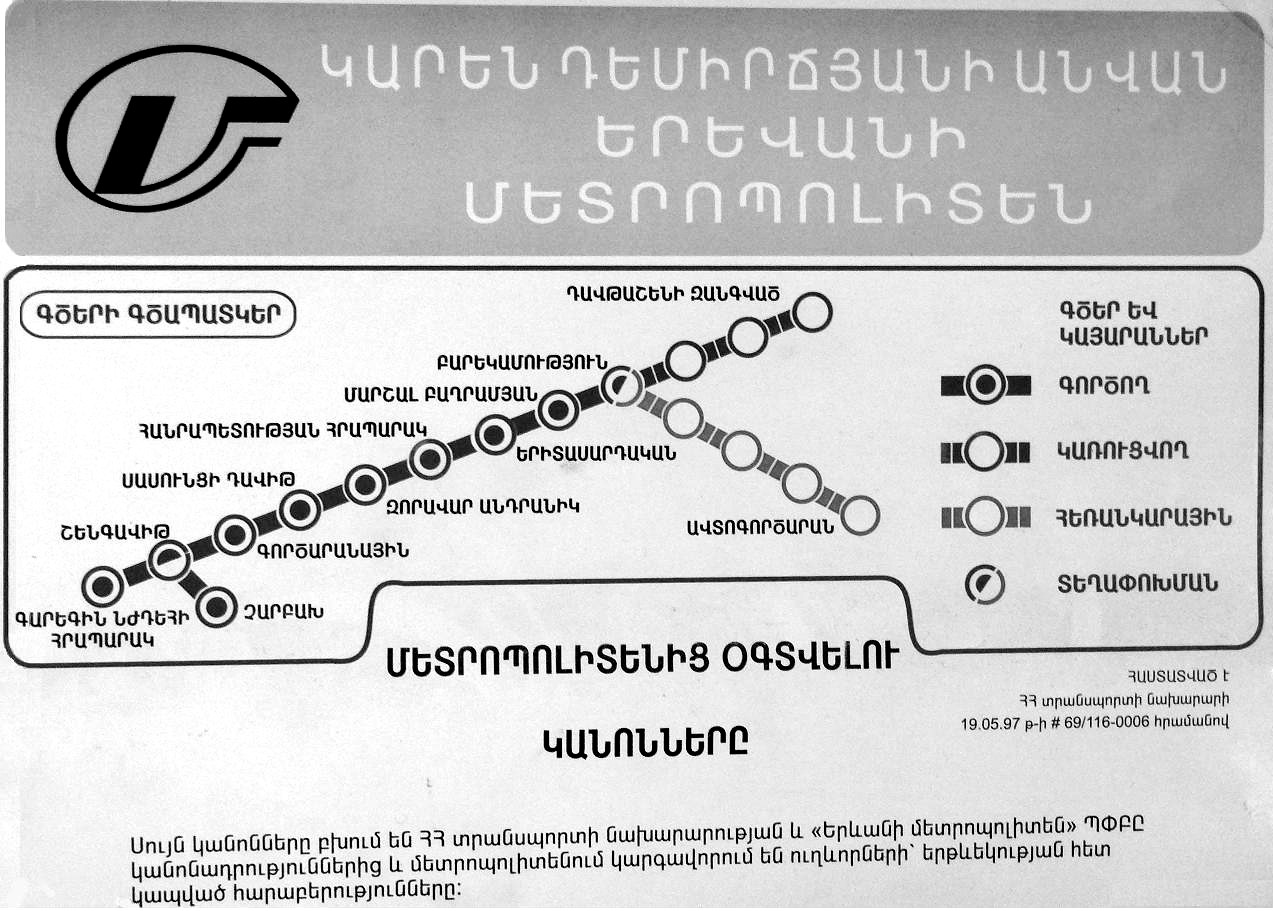
\includegraphics[width=\linewidth]{images/Armenian_Metro}
\end{figure}
\vfill\pagebreak

\begin{assgts}
    \item Assuming Millie takes a train in the correct direction, which will be the first stop after \cmubdata{Shengavit}? Write the name transcribed into English.
    \item After boarding at \cmubdata{Shengavit}, how many stops will it take Millie to get to \cmubdata{Barekamutyun}? Don't include \cmubdata{Shengavit} itself in the number of stops.
    \item What is the name (transcribed into English) of the end station on the short, five-station line that is currently under construction?
\end{assgts}
\end{problem}

\begin{problem}{Ogham}{\nameBNewsome}{\LOYear{\UKLOAbbr}{2021}}
Here are some Irish words written in the Ogham alphabet and their transcriptions in the Latin alphabet (together with their English translations) \OlympiadRandomOrder{}:

\begin{center}
    \begin{tabular}{@{}rc cl@{}}
         \oghamline{\char"1688\char"1693\char"1690\char"168C\char"1686\char"1682\char"1690\char"1689\char"1686}{grá}{love}
         \oghamline{\char"168D\char"168F\char"1690\ \char"168B\char"1691\ \char"1689\char"1686\char"168F\char"1691\char"1694}{teaghlach}{family}
         \oghamline{\char"1685\char"1693\char"1690\char"168F\char"1688}{Éire}{Ireland}
         \oghamline{\char"168C\char"168F\char"1690}{neart}{strength}
         \oghamline{\char"1684\char"1694\char"1691\char"1689\char"1686\char"1690\char"1694\char"1685}{saol}{life}
         \oghamline{\char"1693\char"1694\char"168F\char"1693}{síocháin}{peace}
         \oghamline{\char"1684\char"1690\char"1691\char"1682\vphantom{\char"168F}}{grá mo chroi}{love of my heart}
    \end{tabular}
\end{center}
\begin{assgts}
\item \detcorr
\item Below is the Ogham spelling of the Irish for \texttr{I love you}. Write it down in Latin alphabet transliteration. You can ignore accents for this task.

\begin{center}
    \oghamtext{\char"1688\char"1690\ \char"168B\char"1693\ \char"1694\ \char"1685\char"168C\char"168F\char"1690\ \char"1682\char"1693\char"1690\char"1688}
\end{center}
\end{assgts}
\end{problem}

\begin{problem}{New York Point}{\namePLittell}{\LOYear{\UKLOAbbr}{2011}}
Before the Braille tactile writing system was well established in the United States, the New York Point system (NYP) was widely used in American blind education. NYP was developed in the 1860s by William Bell Walt for the New York Institute for the Blind and was intended to fix the shortcomings he perceived in the French and English Braille standards. The next six decades in blind education became known as the ``War of the Dots", as bitter feuds developed between proponents of this homegrown system and more international Braille-based systems. NYP finally met its end after a series of public hearings convinced educational authorities that there should be a single standard for the entire English-speaking world.

Experts from both sides weighed in on the systems' merits. The proponents of NYP argued that allowing letters to vary in size (from a 2x1 grid to a 2x4 grid, rather than a fixed 3x2 grid) allowed the most frequent letters to use fewer columns, resulting in space (and cost!) savings when publishing texts for the blind. For example, the number of dots needed to write the following names in each system:

\begin{figure}[H]
\pgfplotsset
  {%
    compat=1.11,
    /pgfplots/ybar legend/.style={/pgfplots/legend image code/.code={%
        \draw[##1,/tikz/.cd,bar width=4pt,yshift=-0.2em,bar shift=0pt]
                plot coordinates {(0cm,0.8em)};},
                                }
  } % https://tex.stackexchange.com/a/224677
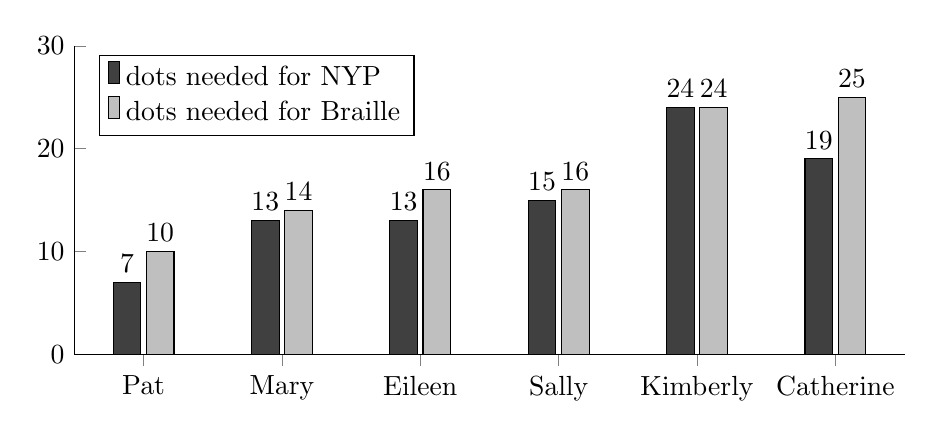
\begin{tikzpicture}
  \begin{axis}[ybar,
        axis lines*=left,
        symbolic x coords = {Pat,Mary,Eileen,Sally,Kimberly,Catherine},
        xtick=data,
        ymin=0,
        ymax=30,
        nodes near coords,
        width=\textwidth,
        height=5.5cm,
        bar width=1em,
        legend pos=north west,
        legend cell align=left
        ]
        \addplot [black,fill=black!75] coordinates {(Pat,7) (Mary,13) (Eileen,13) (Sally,15) (Kimberly,24) (Catherine,19)};
        \addlegendentry{dots needed for NYP}
        
        \addplot [black,fill=black!25] coordinates {(Pat,10) (Mary,14) (Eileen,16) (Sally,16) (Kimberly,24) (Catherine,25)};
        \addlegendentry{dots needed for Braille}
    \end{axis}
\end{tikzpicture}
\end{figure}

\noindent They also pointed out that NYP had a distinct series of capital letters, whereas Braille only had a “capital”\ punctuation mark. 

On the Braille side, experts such as Helen Keller wrote that the NYP capitalization system was unintuitive and confusing (“I have often mistaken \cmubdata{D} for \cmubdata{j}, \cmubdata{I} for \cmubdata{b} and \cmubdata{Y} for double \cmubdata{o} in signatures, and I waste time looking at initial letters over and over again”), and that using Braille allowed her to correspond with blind people from all over the world.

The following 12 words in NYP represent, \OlympiadRandomOrder{}, the names: \cmubdata{Ashley}, \cmubdata{Barb}, \cmubdata{Carl}, \cmubdata{Dave}, \cmubdata{Elena}, \cmubdata{Fred}, \cmubdata{Gerald}, \cmubdata{Heather}, \cmubdata{Ivan}, \cmubdata{Jack}, \cmubdata{Kathy}, \cmubdata{Lisa}. \\

\begin{multicols}{2}
\begin{enumerate}
    \item {\Large \boldmath$\begin{smallmatrix} 
    \bullet & \bullet & \bullet & \bullet \\  & & \bullet &
\end{smallmatrix}$\ \ $\begin{smallmatrix}
  \bullet & \bullet \\  & 
\end{smallmatrix}$\ \ $\begin{smallmatrix}
  \bullet & \bullet \\ \bullet & \bullet
\end{smallmatrix}$\ \ $\begin{smallmatrix}
  & \bullet &  \\ \bullet& & \bullet
\end{smallmatrix}$}

    \item {\Large \boldmath$\begin{smallmatrix} 
    \bullet &  &  &  \\  &\bullet&\bullet & \bullet 
\end{smallmatrix}$\ \ $\begin{smallmatrix}
  \bullet &  \\  \bullet& \bullet
\end{smallmatrix}$\ \ $\begin{smallmatrix}
  \bullet  \\ \,
\end{smallmatrix}$\ \ $\begin{smallmatrix}
  & \\ \bullet & \bullet
\end{smallmatrix}$\ \ $\begin{smallmatrix}
  \bullet & \bullet  \\ & 
\end{smallmatrix}$}

\item {\Large \boldmath$\begin{smallmatrix} 
    \bullet & \bullet & \bullet & \bullet \\ \bullet & &  &
\end{smallmatrix}$\ \ $\begin{smallmatrix}
  \bullet & & \bullet \\  & \bullet &
\end{smallmatrix}$\ \ $\begin{smallmatrix}
  \bullet & \bullet \\  & 
\end{smallmatrix}$\ \ $\begin{smallmatrix}
  &  \\ \bullet& \bullet
\end{smallmatrix}$}
    
\item {\Large \boldmath$\begin{smallmatrix} 
    \bullet & \bullet &  & \bullet \\  & & \bullet &
\end{smallmatrix}$\ \ $\begin{smallmatrix}
  \bullet & \bullet \\  & 
\end{smallmatrix}$\ \ $\begin{smallmatrix}
  & \bullet \\ \bullet & \bullet
\end{smallmatrix}$\ \ $\begin{smallmatrix}
  \bullet &  \\ \bullet& \bullet
\end{smallmatrix}$}

\item {\Large \boldmath$\begin{smallmatrix} 
    \bullet & \bullet & \bullet &  \\  &\bullet &  &\bullet
\end{smallmatrix}$\ \ $\begin{smallmatrix}
  \bullet & \bullet \\  & 
\end{smallmatrix}$\ \ $\begin{smallmatrix}
  \bullet & \bullet & \\  & & \bullet
\end{smallmatrix}$\ \ $\begin{smallmatrix}
  \bullet & \bullet & \bullet \\ & & \bullet
\end{smallmatrix}$}

\item {\Large \boldmath$\begin{smallmatrix} 
     &  & \bullet & \bullet \\ \bullet &\bullet & \bullet &
\end{smallmatrix}$\ \ $\begin{smallmatrix}
  \bullet  \\  \,
\end{smallmatrix}$\ \ $\begin{smallmatrix}
  & \bullet \\ \bullet & \bullet
\end{smallmatrix}$\ \ $\begin{smallmatrix}
  \bullet & \bullet  \\ & 
\end{smallmatrix}$\ \ $\begin{smallmatrix}
  \bullet &   \\ \bullet& \bullet
\end{smallmatrix}$\ \ $\begin{smallmatrix}
  \bullet & \bullet  \\ & \bullet
\end{smallmatrix}$}

\item {\Large \boldmath$\begin{smallmatrix} 
    \bullet &  & \bullet & \bullet \\ \bullet &\bullet&  &
\end{smallmatrix}$\ \ $\begin{smallmatrix}
  \bullet \\  \bullet
\end{smallmatrix}$\ \ $\begin{smallmatrix}
  \bullet & \\ & \bullet
\end{smallmatrix}$\ \ $\begin{smallmatrix}
  \bullet & \bullet  \\  & 
\end{smallmatrix}$}

\item {\Large \boldmath$\begin{smallmatrix} 
    \bullet & \bullet & \bullet &  \\  & &  &\bullet
\end{smallmatrix}$\ \ $\begin{smallmatrix}
  & \bullet \\  \bullet& \bullet
\end{smallmatrix}$\ \ $\begin{smallmatrix}
  \bullet \\ \,
\end{smallmatrix}$\ \ $\begin{smallmatrix}
  \bullet & \bullet \\ & \bullet
\end{smallmatrix}$}

\item {\Large \boldmath$\begin{smallmatrix} 
    & \bullet & \bullet & \bullet & \\  \bullet&\bullet & \bullet &
\end{smallmatrix}$\ \ $\begin{smallmatrix}
  \bullet \\  \, 
\end{smallmatrix}$\ \ $\begin{smallmatrix}
  \bullet & \bullet \\  & 
\end{smallmatrix}$\ \ $\begin{smallmatrix}
 \bullet  & \bullet  \\ \bullet& \bullet
\end{smallmatrix}$\ \ $\begin{smallmatrix}
 \bullet  \\ \,
\end{smallmatrix}$\ \ $\begin{smallmatrix}
  & \bullet  \\ \bullet& \bullet
\end{smallmatrix}$}

\item {\Large \boldmath$\begin{smallmatrix} 
    \bullet & \bullet & \bullet &  \\ \bullet & &  &\bullet
\end{smallmatrix}$\ \ $\begin{smallmatrix}
  \bullet & \bullet \\  & 
\end{smallmatrix}$\ \ $\begin{smallmatrix}
  & \bullet \\ \bullet & \bullet
\end{smallmatrix}$\ \ $\begin{smallmatrix}
  \bullet & \bullet & \bullet  \\ \bullet& & 
\end{smallmatrix}$}

\item {\Large \boldmath$\begin{smallmatrix} 
    \bullet & \bullet & & \\  & & \bullet & \bullet 
\end{smallmatrix}$\ \ $\begin{smallmatrix}
  & \bullet &  \\  \bullet & \bullet & \bullet
\end{smallmatrix}$\ \ $\begin{smallmatrix}
  \bullet & \\ \bullet & \bullet
\end{smallmatrix}$\ \ $\begin{smallmatrix}
  \bullet \\ \, 
\end{smallmatrix}$\ \ $\begin{smallmatrix}
  & \bullet &  \\ \bullet& & \bullet
\end{smallmatrix}$}

\item {\Large \boldmath$\begin{smallmatrix} 
    \bullet & \bullet & \bullet & \bullet \\  & \bullet & &
\end{smallmatrix}$\ \ $\begin{smallmatrix}
  \bullet & \bullet \\  & 
\end{smallmatrix}$\ \ $\begin{smallmatrix}
  \bullet & & \bullet \\ & \bullet &
\end{smallmatrix}$\ \ $\begin{smallmatrix}
  \bullet \\ \,
\end{smallmatrix}$}
\end{enumerate}
\end{multicols}

\begin{assgts}
\item \detcorr
\item Write in NYP: \cmubdata{Billy}, \cmubdata{Ethan}, \cmubdata{Iggie}, \cmubdata{Orson}, \cmubdata{Sasha}, \cmubdata{Tim}.
\end{assgts}
\end{problem}

\begin{problem}{\langnameLepcha}{\nameMChoudhury}{\LOYear{\PLOAbbr}{2015}}
Sikkim state in India has 11 official languages. Amongst these, ten are given below (the eleventh one is English) written in the Lepcha script, as well as in the Latin script:

\begin{center}
    \begin{tabular}{lc@{\hskip0.5in}lc}
        \cmubdata{nepaalii} & \lepchatext{\huge \charstack{\char"1C0D}{\char"1C2C}\char"1C0E\char"1C28\char"1C27\charstack{\char"1C1C}{\char"1C36}} & \cmubdata{newaar} & \lepchatext{\huge \charstack{\char"1C0D}{\char"1C2C}\charstack{\char"1C22}{\char"1C32}\char"1C28}  \\[0.3em]

        \cmubdata{lepchaa} & \lepchatext{\huge \charstack{\char"1C1C}{{\char"1C2C}{\char"1C31}}\char"1C06\char"1C28} & \cmubdata{raai} & \lepchatext{\huge \char"1C1B\char"1C28\char"1C27\char"1C23}  \\[0.3em]

        \cmubdata{sikkim} & \lepchatext{\huge \charstack{\char"1C0C}{{\char"1C2C}{\char"1C30}}\char"1C25\char"1C34\char"1C29\char"1C19\charstack{\char"1C00}{{\char"1C2C}{\char"1C36}}} & \cmubdata{gurung} & \lepchatext{\huge \char"1C03\char"1C2A\char"1C34\char"1C1B\char"1C2A}  \\[0.3em]

        \cmubdata{taamaang} & \lepchatext{\huge \char"1C0A\char"1C28\char"1C34\char"1C15\char"1C28} & \cmubdata{magar} & \lepchatext{\huge \char"1C15\charstack{\char"1C03}{\char"1C32}}  \\[0.3em]

        \cmubdata{liimbu} & \lepchatext{\huge \char"1C27
        \charstack{\charstack{\char"1C1C}{\char"1C2E}}{\raisebox{0.15em}{\char"1C36}}\char"1C13\char"1C2A} & \cmubdata{sunwaar} & \lepchatext{\huge \charstack{\char"1C20}{\char"1C30}\char"1C2A\charstack{\char"1C22}{\char"1C32}\char"1C28}  \\[0.3em]
    \end{tabular}
\end{center}

\begin{assgts}
\item One of the languages above has, in reality, two names, and its name written in the Latin script does not match the name written in the Lepcha script. Its name, transliterated from Lepcha, is \cmubdata{drenzoongkee}. Which language is this?
\item The Lepcha speakers, who call themselves \cmubdata{roong haagiit} (or, in the Lepcha script, \lepchatext{\char"1C34\char"1C29\char"1C1B\ \ \char"1C1D\char"1C28\char"1C27\charstack{\charstack{\char"1C03}{\char"1C33}}{\raisebox{0.15em}{\char"1C36}}}) are composed of four main distinct communities: \lepchatext{\charstack{\char"1C1B}{{\char"1C30}{\char"1C2C}}\char"1C34\char"1C29\char"1C19\char"1C15\char"1C2A}, \lepchatext{\charstack{\char"1C0A}{\char"1C2E}\char"1C28\char"1C34\char"1C20\char"1C28\char"1C15\char"1C2A}, \lepchatext{\char"1C27\char"1C1D\charstack{\char"1C1C}{\char"1C2E}\char"1C28\char"1C15\char"1C2A}, and \lepchatext{\char"1C29\char"1C0E\char"1C25\char"1C15\char"1C2A}. Transcribe these four community names into the Latin script.
\item Sikkim boasts the \cmubdata{Kaangchenzoonggaa}, the third highest peak in the world, which, in Tibetan, means \texttr{the five treasures of the high snow}. Transcribe the name of this peak in Lepcha.
\end{assgts}

\begin{tblsWarning}
Vowel doubling denotes length. \explainch{ch}; \explainng{ng}; \explainv{w}.
\end{tblsWarning}
\end{problem}

\begin{problem}{\langnameArabic\ -- \langnameHebrew}{\nameGParti}{\LOYear{\HKLOAbbr}{2020}}

Arabic and Hebrew are today two different, mutually unintelligible languages. However, they share both grammatical similarities and several lexical correspondences. Besides loanwords (mostly from Arabic to Hebrew) from different historical periods, scholars have identified over a thousand \textit{cognates} (words with a common etymological origin from Proto-Semitic, which is the partially re\-con\-structed common ancestor language spoken around 6,000 years ago).

The two lists below show pairs of cognates, but the pairs are mixed: Arabic on the left, and Hebrew on the right. The first match (1--A) is given for you.

% \begin{center}
    \begin{longtable}{>{\LARGE}crcrc}
        \arbtext{شمس} & 1. & $\xleftrightarrow{\hphantom{Indent}}$ & A. & \LARGE{{שׁמשׁ}}\\[0.3em]
        \arbtext{غضب} & 2. &  & B. & \LARGE{{כּלב}}\\[0.3em]
        \arbtext{ولد} & 3. &  & C. & \LARGE{{מלך}}\\[0.3em]
        \arbtext{أرض} & 4. &  & D. & \LARGE{{עבד}}\\[0.3em]
        \arbtext{بطن} & 5. &  & E. & \LARGE{{ארץ}}\\[0.3em]
        \arbtext{كلب} & 6. &  & F. & \LARGE{{עצב}}\\[0.3em]
        \arbtext{حبل} & 7. &  & G. & \LARGE{{קרן}}\\[0.3em]
        \arbtext{ملك} & 8. &  & H. & \LARGE{{ילד}}\\[0.3em]
        \arbtext{قرن} & 9. &  & I. & \LARGE{{חבל}}\\[0.3em]
        \arbtext{عبد} & 10. &  & J. & \LARGE{{בּטן}}\\[0.3em]
    \end{longtable}
% \end{center}

Thanks to regular and consistent sound changes, we have some easily identifiable patterns. Take for example the following eight words from the list above (transcribed in the Latin script):

\begin{table}[H]
\begin{tabular}{lll lll}
    \lsptoprule
    \langnameArabic & \langnameHebrew & Translation & \langnameArabic & \langnameHebrew & Translation \\
    \cmidrule(r){1-3}\cmidrule(l){4-6}
    \arabhebtr{kalb}{kelev}{dog} & \arabhebtr{shams}{shemesh}{sun} \\
    \arabhebtr{malik}{melekh}{king} & \arabhebtr{qarn}{qeren}{horn} \\
    \arabhebtr{'arḍ}{'erets}{land, earth} & \arabhebtr{ghaḍab}{\textsuperscript{ʕ}etsev}{anger, sadness} \\
    \arabhebtr{\textsuperscript{ʕ}abd}{\textsuperscript{ʕ}eved}{slave} & \arabhebtr{walad}{yeled}{child} \\
    \lspbottomrule
\end{tabular}
\end{table}

\begin{assgts}
    \item What is the transliteration (in both Arabic and Hebrew) of the two word pairs from the lists 1-10 and A-J not included in the table showing transliterations?
    \item The chart below shows a few letters in both scripts with their transliterations. Note that some letters may have different forms depending on the context they appear in. 
    
    \begin{description}[style=nextline]
    \item [\langnameHebrew:] ~ \\
        \begin{tabular}{|c|c|c|c|c|c|}
        \hline 
             \LARGE{{ר}} & \LARGE{{ץ / צ}} & \LARGE{{ע}} & \LARGE{{ן / נ}} & \LARGE{{ךּ / כּ}} & \LARGE{{י}} \\  \hline 
             (1)         & (2)             & (3)         & (4)             & \cmubdata{k}    & (5)         \\  \hline 
        \end{tabular}\medskip\\
        \begin{tabular}{|c|c|c|c|c|c|}
            \hline
             \LARGE{{ט}} & \LARGE{{ח}} & \LARGE{{ד}} & \LARGE{{ב}} & \LARGE{{בּ}} & \LARGE{{א}} \\\hline
             \cmubdata{t} & \cmubdata{ẖ}  & (6) & (7) & \cmubdata{b} & \cmubdata{'} (alef)\\\hline
        \end{tabular}    
    \item[\langnameArabic:] ~ \\
        \begin{tabular}{|@{\hskip0.2em}c@{\hskip0.2em}|c@{\hskip0.2em}|c@{\hskip0.2em}|c@{\hskip0.2em}|c@{\hskip0.2em}|}
        \hline 
            \arbtext{ـط} / \arbtext{ـطـ} / \arbtext{طـ} & \arbtext{ـر} / \arbtext{ر} & \arbtext{ـد} / \arbtext{د} & \arbtext{ـح} / \arbtext{ـحـ} / \arbtext{حـ} & \arbtext{ـب} / \arbtext{ـبـ} / \arbtext{بـ}  \\\hline 
            \cmubdata{ṭ} & (8) & (9) & \cmubdata{ḥ} & (10)  \\ \hline 
        \end{tabular}\medskip\\
        \begin{tabular}{|c@{\hskip0.2em}|@{\hskip0.2em}c@{\hskip0.2em}|c@{\hskip0.2em}|c@{\hskip0.2em}|c@{\hskip0.2em}|c@{\hskip0.2em}|}
        \hline 
            \arbtext{أ} & \arbtext{ـو} / \arbtext{و} & \arbtext{ـن} / \arbtext{ـنـ} / \arbtext{نـ} & \arbtext{ـل} / \arbtext{ـلـ} / \arbtext{لـ} & \arbtext{ـك} / \arbtext{ـكـ} / \arbtext{كـ} & \arbtext{ض} \\\hline 
            \cmubdata{'} (alif) & (11) & (12) & (13) & (14) & (15)  \\ \hline 
        \end{tabular}
\end{description}
    \item[] Fill in the gaps (1--15).
    
    \item Pair the matching cognates 2-10 and B-J from the first list (words transcribed in Arabic and Hebrew).
    \item If \texttr{thousand} in Arabic is \arbtext{ألف} and the final letter \cmubdata{f} in Hebrew is \mbox{ף}, what is the transliteration of {{אלף}} – also meaning \texttr{thousand} in Hebrew?
\end{assgts}

\begin{tblsWarning}
The apostrophe (') in both languages represents a glottal stop /ʔ/. In Arabic it is written by a \textit{hamza}, which often `sits' on top of an \textit{alif}; in Hebrew, it is represented by an \textit{alef} and often omitted in pronunciation. Here, you should just consider it a consonant and treat it like you would treat any other consonant!

The symbol \textsuperscript{ʕ} represents a voiced pharyngeal fricative /ʕ/, which is an odd sound made by contracting the muscles in the throat. It gives Arabic its unique flavour we can easily hear. In Modern Hebrew, it is silent and almost only ever appears in writing. Just think of it as an ordinary consonant!
\end{tblsWarning}

\end{problem}

\begin{problem}{\langnameJavanese}{\nameTHLee}{\LOYear{\NACLOAbbr}{2016}}
Here are some Javanese words in the Javanese script, Latin script, and their English translations:

\begin{center}
\begin{longtable}{rccc}
     \javaneseline{\javtext{\char"A9A5\char"A9BC\char"A99A\char"A98F\char"A9B6\char"A9A0\char"A9C0}}{penyakit}{disease}
     \javaneseline{\javtext{\char"A986\char"A981\ \char"A992\char"A9BF\char"A9B6\char"A9B1\char"A9C0}}{Inggris}{England}
     \javaneseline{\begin{tabular}{c}
          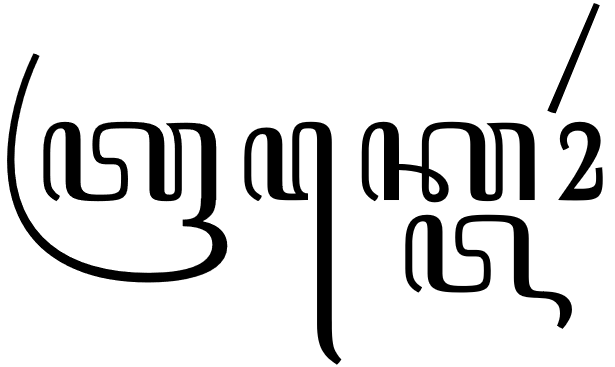
\includegraphics[width = 7em]{images/Java-stacked/3.png} 
     \end{tabular}}{traktor}{tractor}
     \javaneseline{\begin{tabular}{c}
          
\includegraphics[width = 6.5em]{images/Java-stacked/4.png} 
     \end{tabular}}{panyumbang}{donor}
     \javaneseline{\begin{tabular}{c}
          
\includegraphics[width = 8em]{images/Java-stacked/5.png} 
     \end{tabular}}{rembulan}{moon}
     \javaneseline{\begin{tabular}{c}
          
\includegraphics[width = 6.5em]{images/Java-stacked/6.png} 
     \end{tabular}}{tansah}{always}
     \javaneseline{\javtext{\char"A984\char"A9BA\hspace{0.4em} \char"A9A9\char"A9AB\char"A9B6\char"A98F}}{Amérika}{America}
     \javaneseline{\javtext{\char"A994\char"A9BD\char"A9A7\char"A9B8\char"A9A0\char"A9C0}}{ngrebut}{to grab}
     \javaneseline{\javtext{\char"A9B2\char"A9B6\char"A9A7\char"A9B8\char"A9BA\hspace{0.65em}\char"A98F\char"A9B4\char"A9A0}}{ibukota}{capital}
     \javaneseline{\begin{tabular}{c}
          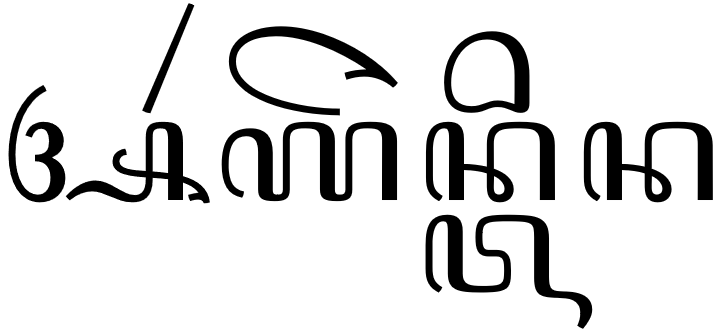
\includegraphics[width = 8em]{images/Java-stacked/10.png} 
     \end{tabular}}{Argentina}{Argentina}
     \javaneseline{\javtext{\char"A9B1\char"A9BD\char"A9BA\hspace{0.65em}\char"A994\char"A9BA\hspace{0.65em}\char"A994}}{srengéngé}{sun}
     \javaneseline{\begin{tabular}{c}
          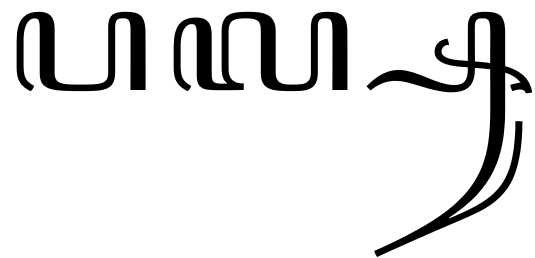
\includegraphics[width = 6em]{images/Java-stacked/12.png} 
     \end{tabular}}{palsu}{false}
     \javaneseline{\javtext{\char"A989\char"A989\char"A981\char"A992\char"A9A4\char"A9C0}}{rerenggan}{decoration}
     \javaneseline{\javtext{\char"A9B2\char"A981\char"A9B1\char"A9AD\char"A9C0}}{angsal}{to acquire}
     \javaneseline{\javtext{\char"A9B2\hspace{-0.3em}\char"A9B6\hspace{0.5em}\char"A981\hspace{-0.2em}\char"A992\char"A9B6\char"A983}}{inggih}{yes}
     \javaneseline{\javtext{\char"A98F\char"A9BC\char"A989\char"A9A5\char"A9C0}}{\pbblank}{often}
     \javaneseline{\begin{tabular}{c}
          
\includegraphics[width = 8em]{images/Java-stacked/17.png} 
     \end{tabular}}{\pbblank}{letter, script}
     \javaneseline{\begin{tabular}{c}
          
\includegraphics[width = 6em]{images/Java-stacked/18.png} 
     \end{tabular}}{\pbblank}{to unload}
     \javaneseline{\begin{tabular}{c}
          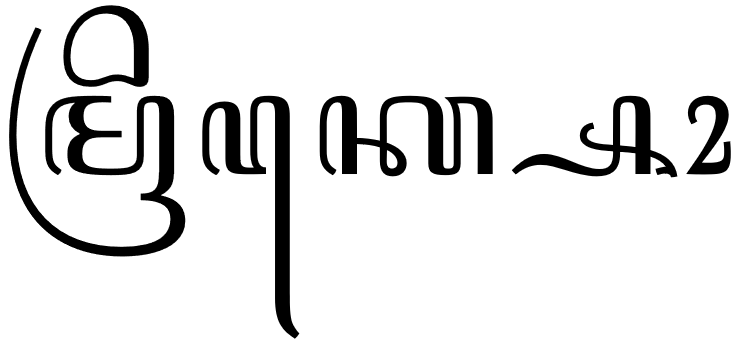
\includegraphics[width = 8em]{images/Java-stacked/19.png} 
     \end{tabular}}{\pbblank}{to examine}
     \javaneseline{\javtext{\char"A9A9\char"A9B8\char"A9AB\char"A9B8\char"A994\char"A9BA\hspace{0.65em}\char"A98F}}{\pbblank}{to cancel}
     \javaneseline{\pbblank}{nyolong}{to steal}
     \javaneseline{\pbblank}{sepalih}{half}
     \javaneseline{\pbblank}{trengginas}{lively}
     \javaneseline{\pbblank}{Antartika}{Antarctica}
     \javaneseline{\pbblank}{Istanbul}{Istanbul}
\end{longtable}
\end{center}

\begin{assgts}
\item \fillblanks
\end{assgts}
\begin{tblsWarning} 
\cmubdata{ny} and \cmubdata{ng} are consonants; \cmubdata{é} is a vowel.
\end{tblsWarning}
\end{problem}

\begin{problem}{\langnameThai}{\nameSDmitrenko}{\LOYear{\MSKAbbr}{2001}}
Here are some Thai words written in the Thai script and their Latin transcriptions (together with their English translations) given \OlympiadRandomOrder{}:
\begin{enumerate}

    \begin{multicols}{5}
        \item \thaitext{หวาย}
        \item \thaitext{ท่าน}
        \item \thaitext{วาย}
        \item \thaitext{ว่าย}
        \item \thaitext{กาย}
        \item \thaitext{ทัน}
        \item \thaitext{กาว}
        \item \thaitext{ถาด}
        \item \thaitext{ถาก}
        \item \thaitext{วัย}
        \item \thaitext{หลาว}
        \item \thaitext{ทาน}
        \item \thaitext{หลัง}
        \item \thaitext{ลาว}
        \item[] \quad 
    \end{multicols}
\end{enumerate}

\begin{center}
    \begin{tabular}{rll@{\hskip1in}rll}
        A. & \pbsv{tʰà:k}{to clear (a field)} & H. & \pbsv{ka:w}{glue} \\[0.3em]
        B. & \pbsv{vâ:y}{to swim} & I. & \pbsv{la:w}{Laotian} \\[0.3em]
        C. & \pbsv{lǎ:w}{javelin} & J. & \pbsv{tʰâ:n}{you (formal)} \\[0.3em]
        D. & \pbsv{va:y}{to end} & K. & \pbsv{tʰa:n}{charity} \\[0.3em]
        E. & \pbsv{vǎ:y}{rattan} & L. & \pbsv{vay}{age} \\[0.3em]
        F. & \pbsv{tʰan}{to have time} & M. & \pbsv{tʰà:t}{tray} \\[0.3em]
        G. & \pbsv{lǎŋ}{back} & N. & \pbsv{ka:y}{body} \\[0.3em]
    \end{tabular}
\end{center}
\begin{assgts}
\item \detcorr
\item \taskWriteIn{\langnameThai}:

\begin{center}
    \begin{tabular}{rll@{\hskip1in}rll}
         15. & \pbsv{vǎ:n}{sweet} & 17. & \pbsv{tʰàk}{to knit} \\[0.3em] 
         16. & \pbsv{ya:ŋ}{rubber} & 18. & \pbsv{vâ:w}{kite} \\[0.3em] 
    \end{tabular}
\end{center}
\end{assgts}

\begin{tblsWarning}
A colon (\cmubdata{:}) after a vowel indicates length. The marks above vowels denote tones. This problem features four tones: medium (\cmubdata{a}), rising (\cmubdata{ǎ}), falling (\cmubdata{â}), low (\cmubdata{à}).

\cmubdata{tʰ} and \cmubdata{ŋ} are consonants.
\end{tblsWarning}

\end{problem}

\hypertarget{solutions-of-practice-problems}{%
\section{Solutions of practice problems}}

\begin{practiceproblemsolution}{2.5. \langnameArmenian}

\begin{solutions}[label=Solution 2.5\alph*]
    \item \cmubdata{Gortsaranayin}
    \item 7
    \item \cmubdata{Avtogortsaran} (the character resembling the letter S can be inferred to mean \cmubdata{t} from the title of the map, where the last word is \cmubdata{metropoliten}).
\end{solutions}

\end{practiceproblemsolution}

\pagebreak
\begin{practiceproblemsolution}{2.6. Ogham}

\begin{solutions}[label=Solution 2.6\alph*]
    \item \begin{enumerate}
        \begin{multicols}{7}
            \item B
            \item G
            \item D
            \item A
            \item F
            \item C
            \item E
        \end{multicols}
    \end{enumerate}
    \item \cmubdata{ta me i ngra leat} (in reality it is \cmubdata{Tá mé i ngrá leat}).
\end{solutions}

\rules

We can classify the characters depending on the number of dots or lines as well as their position or direction (vertical or diagonal, above or below the horizontal line):

\begin{table}[H]
    \begin{tabular}{l *5{c}}
    \lsptoprule
 & 1 line & 2 lines & 3 lines & 4 lines & 5 lines \\\midrule
vertical, below & & \cmubdata{l} &  & \cmubdata{s} & \cmubdata{n} \\
vertical, above & \cmubdata{h} &  & \cmubdata{t} & \cmubdata{c} &  \\
diagonal & \cmubdata{m} & \cmubdata{g} &  &  & \cmubdata{r} \\
dots & \cmubdata{a} & \cmubdata{o} &  & \cmubdata{e} & \cmubdata{i}\\
\lspbottomrule
\end{tabular}
\end{table}

The accents are not marked (\cmubdata{á} = \cmubdata{a}).
\end{practiceproblemsolution}



\begin{practiceproblemsolution}{2.7. New York Point}

\begin{solutions}[label=Solution 2.7\alph*]
    \item \begin{enumerate}\largerpage[2]

    \begin{multicols}{4}
        \item \cmubdata{Kathy}
        \item \cmubdata{Elena}
        \item \cmubdata{Ivan}
        \item \cmubdata{Carl}
        \item \cmubdata{Jack}
        \item \cmubdata{Gerald}
        \item \cmubdata{Lisa}
        \item \cmubdata{Fred}
        \item \cmubdata{Heather}
        \item \cmubdata{Barb}
        \item \cmubdata{Ashley}
        \item \cmubdata{Dave}
    \end{multicols}
    \end{enumerate}
    \item
    \begin{tabular}[t]{lcl}
         \cmubdata{Billy} & -- & {\Large \boldmath$\begin{smallmatrix}
    \bullet & \bullet & \bullet &  \\  \bullet& &  &\bullet
\end{smallmatrix}$\ \ \boldmath$\begin{smallmatrix}
    \bullet \\  \bullet\end{smallmatrix}$\ \ \boldmath$\begin{smallmatrix}
    \bullet &\\  \bullet&\bullet\end{smallmatrix}$\ \ \boldmath$\begin{smallmatrix}
    \bullet & \\  \bullet&\bullet\end{smallmatrix}$\ \ \boldmath$\begin{smallmatrix}
    &\bullet& \\  \bullet&&\bullet\end{smallmatrix}$}\\ [0.5em]
         \cmubdata{Ethan} & -- & {\Large \boldmath$\begin{smallmatrix}
    \bullet &  &  &  \\  &\bullet & \bullet &\bullet
\end{smallmatrix}$\ \ \boldmath$\begin{smallmatrix}
    \bullet &\bullet  \\  \bullet&\bullet\end{smallmatrix}$\ \ \boldmath$\begin{smallmatrix}
    \bullet&\bullet \\  &\end{smallmatrix}$\ \ \boldmath$\begin{smallmatrix}
    & \\  \bullet&\bullet\end{smallmatrix}$}\\[0.5em]
         \cmubdata{Iggie} & -- & {\Large \boldmath$\begin{smallmatrix}
    \bullet & \bullet & \bullet & \bullet \\  \bullet &&
\end{smallmatrix}$\ \ \boldmath$\begin{smallmatrix}
    &&\bullet \\ \bullet&\bullet&\bullet\end{smallmatrix}$\ \ \boldmath$\begin{smallmatrix}
    &&\bullet \\ \bullet&\bullet&\bullet\end{smallmatrix}$\ \ \boldmath$\begin{smallmatrix}
    \bullet \\  \bullet\end{smallmatrix}$\ \ \boldmath$\begin{smallmatrix}
    \bullet \\  \end{smallmatrix}$}\\[0.5em]
    \cmubdata{Orson} & -- & {\Large\boldmath$\begin{smallmatrix}
    &\bullet&& \\  \bullet&&\bullet&\bullet\end{smallmatrix}$\ \ \boldmath$\begin{smallmatrix}
    &\bullet \\  \bullet&\bullet\end{smallmatrix}$\ \ \boldmath$\begin{smallmatrix}
    \bullet& \\  &\bullet\end{smallmatrix}$\ \ \boldmath$\begin{smallmatrix}
    &\bullet \\  \bullet&\end{smallmatrix}$\ \ \boldmath$\begin{smallmatrix}
    &\\\bullet&\bullet\end{smallmatrix}$}\\[0.5em]
         \cmubdata{Sasha} & -- & {\Large \boldmath$\begin{smallmatrix}
    \bullet && \bullet & \bullet  \\  &\bullet &  &
\end{smallmatrix}$\ \ \boldmath$\begin{smallmatrix}
    \bullet&\bullet \\  &\end{smallmatrix}$\ \ \boldmath$\begin{smallmatrix}
    &\bullet& \\ \bullet&\bullet&\bullet\end{smallmatrix}$\ \ \boldmath$\begin{smallmatrix}
    \bullet&\bullet \\  &\end{smallmatrix}$}\\[0.5em]
         \cmubdata{Tim} & -- & {\Large \boldmath$\begin{smallmatrix}
    & \bullet & \bullet & \bullet  \\  \bullet &&  &
\end{smallmatrix}$\ \ \boldmath$\begin{smallmatrix}
    \bullet \\  \bullet\end{smallmatrix}$\ \ \boldmath$\begin{smallmatrix}
    \bullet&\bullet \\  \bullet&\end{smallmatrix}$}\\
    \end{tabular}
\end{solutions}

\rules

Forming the capital letter: all capital letters are four columns long and are formed by appending dots to the lowercase letter until it is four columns long, according to the following pattern:

\begin{itemize}
    \item If the last column of the lowercase letter has a dot in the upper row, add the extra dots on the lower row.
    \item If the last column of the lowercase letter has a dot in the lower row or both dots, add the extra dots on the upper row.
\end{itemize}
\end{practiceproblemsolution}

\begin{discussion}
\begin{sloppypar}
Figuring out the character for \cmubdata{o}: in the introduction it is mentioned that \cmubdata{Y} ({\Large \boldmath$\begin{smallmatrix}
    &\bullet&&\bullet&  \\  \bullet&&\bullet&
\end{smallmatrix}$}) can be mistaken for a double \cmubdata{o}, and \cmubdata{Y} is formed by the same pattern repeated twice, so that pattern must represent the letter \cmubdata{o} ({\Large \boldmath$\begin{smallmatrix} 
   & \bullet  \\  \bullet& 
\end{smallmatrix}$}).
\end{sloppypar}

Figuring out the characters for \cmubdata{t} and \cmubdata{m}: based on the graph given in the introduction, we can deduce that \cmubdata{t} must contain a single dot (\cmubdata{Pat} has seven dots, \cmubdata{a} is two dots and \cmubdata{P}, since it is uppercase, must have at least four dots). Since we already know that \cmubdata{e} is {\Large \boldmath$\begin{smallmatrix}
    \bullet  \\   
\end{smallmatrix}$}, \cmubdata{t} can only be {\Large \boldmath$\begin{smallmatrix} 
     \\  \bullet 
\end{smallmatrix}$}.

From the graph, we deduce that \cmubdata{M} has five dots and \cmubdata{m} three, therefore the three dots must be distributed on only two columns (since two columns are needed for the extra dots to form the uppercase). There are four options ({\Large \boldmath$\begin{smallmatrix}
    &\bullet  \\  \bullet&\bullet 
\end{smallmatrix}$}, {\Large \boldmath$\begin{smallmatrix} 
    \bullet&\bullet  \\  \bullet &
\end{smallmatrix}$} , {\Large \boldmath$\begin{smallmatrix} 
    \bullet&  \\  \bullet &\bullet
\end{smallmatrix}$} , {\Large \boldmath$\begin{smallmatrix} 
    \bullet&\bullet  \\  &\bullet 
\end{smallmatrix}$}). Since three of the characters are already used ({\Large \boldmath$\begin{smallmatrix} 
    &\bullet  \\  \bullet&\bullet 
\end{smallmatrix}$} = \cmubdata{r}, {\Large \boldmath$\begin{smallmatrix} 
    \bullet&  \\  \bullet &\bullet
\end{smallmatrix}$} = \cmubdata{l}, {\Large \boldmath$\begin{smallmatrix} 
    \bullet&\bullet  \\  &\bullet 
\end{smallmatrix}$} = \cmubdata{d}), there is only one option left to place the dots ({\Large \boldmath$\begin{smallmatrix} 
    \bullet&\bullet  \\  \bullet &
\end{smallmatrix}$}) such as the final pattern does not coincide with other letters.
\end{discussion}


\begin{practiceproblemsolution}{2.8. \langnameLepcha}

\begin{solutions}[label=Solution 2.8\alph*]
    \item Sikkim language
    \item \cmubdata{renzoongmu} \hfill \cmubdata{taamsaangmu} \hfill \cmubdata{hilaammu} \hfill \cmubdata{proomu}
    \item \lepchatext{\char"1C34\char"1C00\char"1C28\charstack{\char"1C06}{{\char"1C2C}{\char"1C30}}\char"1C34\char"1C29\char"1C19\char"1C03\char"1C28}
\end{solutions}

\rules
\begin{itemize}
    \item Abugida script, left-to-right.
    \item Consonants at the beginning of the syllable:

    \begin{center}
        \begin{tabular}{cccccccc}
            \lepchatext{\char"1C23} & \lepchatext{\char"1C13} & \lepchatext{\char"1C0C} & \lepchatext{\char"1C03} & \lepchatext{\char"1C1D} & \lepchatext{\char"1C06} & \lepchatext{\char"1C00} & \lepchatext{\char"1C1C} \\
            $\varnothing$ & \cmubdata{b} & \cmubdata{d} & \cmubdata{g} & \cmubdata{h} & \cmubdata{ch} & \cmubdata{k} & \cmubdata{l}\\\addlinespace
            \lepchatext{\char"1C15} & \lepchatext{\char"1C0D} & \lepchatext{\char"1C0E} & \lepchatext{\char"1C1B} & \lepchatext{\char"1C20} & \lepchatext{\char"1C0A} & \lepchatext{\char"1C22} & \lepchatext{\char"1C19} \\
            \cmubdata{m} & \cmubdata{n} & \cmubdata{p} & \cmubdata{r} & \cmubdata{s} & \cmubdata{t} & \cmubdata{w} & \cmubdata{z}\\
        \end{tabular}
    \end{center}

    \item Vowels are marked by diacritics. The default vowel is \cmubdata{a}.

    \begin{center}
        \begin{tabular}{cccccccc}
            \lepchatext{\char"25CC} & \lepchatext{\char"25CC\char"1C28} & \lepchatext{\charstack{\char"25CC}{\char"1C2C}} & \lepchatext{\charstack{\char"25CC}{{\char"1C2C}{\char"1C36}}} & \lepchatext{\char"1C27\char"25CC} & \lepchatext{\char"1C27\charstack{\char"25CC}{\char"1C36}} & \lepchatext{\char"1C29\char"25CC} & \lepchatext{\char"25CC\char"1C2A} \\
            \cmubdata{a} & \cmubdata{aa} & \cmubdata{e} & \cmubdata{ee} & \cmubdata{i} & \cmubdata{ii} & \cmubdata{oo} & \cmubdata{u}\\
        \end{tabular}
    \end{center}

    \item Consonants at the end of the syllable (codas) are also marked by diacritics:

    \begin{center}
        \begin{tabular}{cccccc}
            \lepchatext{\charstack{\char"25CC}{\char"1C2E}} & \lepchatext{\charstack{\char"25CC}{\char"1C30}} &  \lepchatext{\char"1C34\char"25CC} & \lepchatext{\charstack{\char"25CC}{\char"1C31}} & \lepchatext{\charstack{\char"25CC}{\char"1C32}} & \lepchatext{\charstack{\char"25CC}{\char"1C33}} \\
            \cmubdata{-m} & \cmubdata{-n} & \cmubdata{-ng} & \cmubdata{-p} & \cmubdata{-r} & \cmubdata{-t}\\
        \end{tabular}
    \end{center}
    \item If the syllable onset has the structure $C$\cmubdata{r}, that \cmubdata{r} is marked as \lepchatext{\char"25CC\char"1C25}. Compare:

    \begin{center}
        \begin{tabular}{ccc}
             \lepchatext{\char"1C00\char"1C25} & \lepchatext{\charstack{\char"1C00}{\char"1C32}} & \lepchatext{\charstack{\char"1C00}{\char"1C32}\char"1C25} \\
             \cmubdata{k\textbf{r}a} & \cmubdata{ka\textbf{r}} & \cmubdata{k\textbf{r}a\textbf{r}}
        \end{tabular}
    \end{center}
\end{itemize}
\end{practiceproblemsolution}


\begin{practiceproblemsolution}{2.9. Arabic and Hebrew}\largerpage[1.5]

\begin{solutions}[label=Solution 2.9\alph*]
    \item \cmubdata{ḥabl} \rightarrow\ \cmubdata{ẖevel} \\ \cmubdata{baṭn} \rightarrow\ \cmubdata{beten}
\end{solutions}

    \note{In Hebrew all vowels shown are \cmubdata{e}. In Arabic it is impossible to deduce the vowels based on the data, so alternative versions are also accepted (such as \cmubdata{ḥabal} or \cmubdata{ḥabil}).}
    
\begin{solutions}[label=Solution 2.9\alph*, resume]
    \item \largerpage
    \begin{multicols}{3}
    \begin{enumerate}[label = (\arabic*)]
            \item \cmubdata{r}
            \item \cmubdata{ts}
            \item \cmubdata{\textsuperscript{ʕ}} (ayin)
            \item \cmubdata{n}
            \item \cmubdata{y}
            \item \cmubdata{d}
            \item \cmubdata{v}
            \item \cmubdata{r}
            \item \cmubdata{d}
            \item \cmubdata{b}
            \item \cmubdata{w}
            \item \cmubdata{n}
            \item \cmubdata{l}
            \item \cmubdata{k}
            \item \cmubdata{ḍ}
        \end{enumerate}
    \end{multicols}
    \item \begin{enumerate}
        \begin{multicols}{5}
            \item A
            \item F
            \item H
            \item E
            \item J
            \item B
            \item I
            \item C
            \item G
            \item D
        \end{multicols}
    \end{enumerate}
    \item \cmubdata{'elef}
\end{solutions}

\end{practiceproblemsolution}
\pagebreak
\begin{practiceproblemsolution}{2.10. \langnameJavanese}

\begin{solutions}[label=Solution 2.10\alph*]
    \item
    \begin{enumerate}[label = (\arabic*)]

    \begin{multicols}{2}
        \item \cmubdata{kerep}
        \item \cmubdata{aksara}
        \item \cmubdata{mbongkar}
        \item \cmubdata{mrikso}
        \item \cmubdata{murungaké}
        \item \javtext{\char"A9BA\hspace{0.65em}\char"A99A\char"A9B4\char"A9BA\hspace{0.65em}\char"A9AD\char"A981\char"A9B4}
        \item \javtext{\char"A9B1\char"A9BC\char"A9A5\char"A9AD\char"A9B6\char"A983}
        \item \javtext{\char"A9A0\char"A9BD\char"A981\char"A992\char"A9B6\char"A9A4\char"A9B1\char"A9C0}
        \item \begin{tabular}{@{}l@{}}
             
\includegraphics[width = 9em]{images/Java-stacked/sol9.png}
        \end{tabular}
        \item \begin{tabular}{@{}l@{}}
             
\includegraphics[width = 9em]{images/Java-stacked/sol10.png}
        \end{tabular}
    \end{multicols}
    \end{enumerate}
\end{solutions}

\rules
\begin{itemize}
    \item Abugida script, left-to-right, with the default vowel \cmubdata{a}.
    \item Syllables have the structure $C_1(C_2)V(C_3)$, taking into account the following syllabification rules:
    \begin{itemize}

        \item $...VC^aC^bV... \rightarrow\ ...VC^a_3-C^b_1V...$ if $C^a$ is \cmubdata{ng}, \cmubdata{h}, or \cmubdata{r};
        \item $...VC^aC^bV... \rightarrow\ ...V-C^a_1C^b_1V...$ otherwise;
    \end{itemize}
    \item $C_1$

    \begin{center}
        \begin{tabular}{ccccccc}
            \javtext{\char"A9B2} & \javtext{\char"A9A7} & \javtext{\char"A992} & \javtext{\char"A98F} & \javtext{\char"A9AD} & \javtext{\char"A9A9} & \javtext{\char"A9A4} \\
            $\varnothing$ & \cmubdata{b} & \cmubdata{g} & \cmubdata{k} & \cmubdata{l} & \cmubdata{m} & \cmubdata{n} \\ &&&&&&\\

            \javtext{\char"A994} & \javtext{\char"A99A} & \javtext{\char"A9A5} & \javtext{\char"A9AB} & \javtext{\char"A9B1} & \javtext{\char"A9A0} &  \\
            \cmubdata{ng} &\cmubdata{ny} & \cmubdata{p} & \cmubdata{r} & \cmubdata{s} & \cmubdata{t} &  \\
        \end{tabular}
    \end{center}
    
\end{itemize}\largerpage[1.5]
    \note{The combination \cmubdata{re} has its own character: \javtext{\char"A989}}
\begin{itemize}
    
    \item The vowel change is shown using diacritics:

    \begin{center}
        \begin{tabular}{cccccc}
            \javtext{\char"25CC} & \javtext{\char"25CC\char"A9BC} & \javtext{\char"A9BA\hspace{0.6em}\char"25CC} & \javtext{\char"25CC\char"A9B6} & \javtext{\char"A9BA\hspace{0.6em}\char"25CC\char"A9B4} & \javtext{\char"25CC\char"A9B8}    \\
            \cmubdata{$C$a} & \cmubdata{$C$e} & \cmubdata{$C$é} & \cmubdata{$C$i} & \cmubdata{$C$o} & \cmubdata{$C$u}\\
        \end{tabular}
    \end{center}
    
    \item $C_2$:\footnote{In fact, this special form of the consonant marks the fact that the vowel of the preceding consonant is deleted.}

    \begin{center}
        \begin{tabular}{ccccc}
              \begin{tabular}{@{}c@{}}
                
\includegraphics[width=2em]{images/Java-stacked/b-stack.png}
              \end{tabular} & \javtext{\char"25CC\char"A9BF} & \javtext{\char"25CC\char"A9BD} & \begin{tabular}{@{}c@{}}
                
\includegraphics[width=3em]{images/Java-stacked/s-stack.png}
              \end{tabular} & \begin{tabular}{@{}c@{}}
                
\includegraphics[width=2em]{images/Java-stacked/t-stack.png}
              \end{tabular}
              \\
             \cmubdata{b} & \hphantom{abc}\cmubdata{r}\hphantom{abc} & \cmubdata{re} & \cmubdata{s} & \cmubdata{t}
        \end{tabular}
    \end{center}
    \item $C_3$:

    \begin{center}
        \begin{tabular}{cccc}
            \javtext{\char"25CC\char"A981} & \javtext{\char"25CC\char"A983} & \javtext{\char"25CC\char"A982} & \javtext{C\char"A9C0}\\
            \cmubdata{ng} & \cmubdata{h} & \cmubdata{r} & else (\cmubdata{C})\footnotemark{}\\
        \end{tabular} \footnotetext{This is basically the vowel-removing mark, showing that the previous consonant does not have a vowel.}
    \end{center}
    \item Special characters for capital letters:

    \begin{center}
        \begin{tabular}{cc}
              \javtext{\char"A984} & \javtext{\char"A986}
              \\
             \cmubdata{A} & \cmubdata{I}
        \end{tabular}
    \end{center}
\end{itemize}

\end{practiceproblemsolution}

\begin{practiceproblemsolution}{2.11. \langnameThai}

\begin{solutions}[label=Solution 2.11\alph*]
    \item \begin{enumerate}

        \begin{multicols}{7}
            \item E
            \item J
            \item D
            \item B
            \item N
            \item F
            \item H
            \item M
            \item A
            \item L
            \item C
            \item K
            \item G
            \item I
        \end{multicols}
    \end{enumerate}
    \item \begin{enumerate}[resume]

        \begin{multicols}{4}
            \item \thaitext{หวาน}
            \item \thaitext{ยาง}
            \item \thaitext{ถัก}
            \item \thaitext{ว่าว}
        \end{multicols}
        \end{enumerate}
\end{solutions}

\rules
\begin{itemize}
    \item Writing direction from left to right.
    \item The character \thaitext{ว} represents two consonants: \cmubdata{v}, if in the beginning of the word; and \cmubdata{w}, if at the end of the word.
    \item The sound \cmubdata{t\textsuperscript{h}} corresponds to two Thai characters: \thaitext{ท} and \thaitext{ถ}. The latter is used to mark the low tone.
    \item Vowels: \cmubdata{a} = \thaitext{\char"25CC\char"0E31} (placed on the first consonant), \cmubdata{a:} = \thaitext{า}
    \item Tone:
    \begin{itemize}

        \item Medium -- default tone (unmarked);
        \item Rising -- \thaitext{ห} placed at the beginning of the word;
        \item Falling -- \thaitext{\char"25CC\char"0E48} placed on the first consonant;
        \item Low -- appears only in words starting with \cmubdata{tʰ}. In this case, the tone is marked by using the character \thaitext{ถ} to mark the consonant \cmubdata{tʰ} (rather than \thaitext{ท}).
    \end{itemize}
\end{itemize}
\end{practiceproblemsolution}

\begin{discussion}

The way that the Thai writing system represents tone is very complex. To know which tone to pronounce the syllable with, we need to know the initial consonant and the type of syllable. Initial consonants are split into three classes: low, medium (mid), and high, while the syllables are either ``live" (ending in \cmubdata{n}, \cmubdata{m}, \cmubdata{ŋ}, \cmubdata{w}, \cmubdata{y}) or ``dead" (ending in \cmubdata{p}, \cmubdata{t}, \cmubdata{k}). Moreover, there are some diacritics which may be added to further modify the tone. The following table details the rules relevant to the data in the problem:

\begin{table}[H]
    \begin{tabular}{ccccc}
    \lsptoprule
                 &               & \multicolumn{3}{c}{Type of first consonant} \\\cmidrule(lr){3-5}
     Diacritics  & Syllable type & \textit{low} & \textit{mid} & \textit{high} \\ \midrule 
    no mark      & \textit{live}         & medium (\cmubdata{a}) & medium (\cmubdata{a}) & rising (\cmubdata{\v{a}}) \\
    no mark      & \textit{dead}         & * & low (\cmubdata{à}) & low (\cmubdata{à}) \\  
    \thaitext{\char"25CC\char"0E48} & \textit{live}/\textit{dead}   & falling (\cmubdata{â}) & low (\cmubdata{à})   & low (\cmubdata{à})\\
     \lspbottomrule
    \end{tabular}
\footnotetext{* The choice of tone further depends on the vowel length: if the vowel is long, the syllable will have falling (\cmubdata{â}) tone; if the vowel is short, the syllable will have high (\cmubdata{á}) tone.}
\end{table}


Most words in the problem start with \textit{low} consonants (\thaitext{ล}, \thaitext{ท}, \thaitext{ว}, \thaitext{ล}). There is a single \textit{mid} consonant at the beginning of the words (\cmubdata{k} = \thaitext{ก}), but, since this one only appears in \textit{live} syllables, its tone is identical to that of a syllable starting with a \textit{low} consonant.

Most Thai consonants have two forms: a low form and a high form (in the problem we have the consonant \cmubdata{tʰ}, which, in its low form, is written as \thaitext{ท}, while in its high form becomes \thaitext{ถ}). If some consonants do not have two different characters to differentiate between low and high, a low consonant can become high by adding the character \thaitext{ห} before it (the character represents the high consonant \cmubdata{h}, but it is not pronounced).

Based on this information, the rules in our problem can be explained as follows:

\begin{itemize}
    \item the default tone is the medium one because most of the words contain live syllables and start with a low or mid consonant.
    \item the falling tone is shown by the diacritic \thaitext{\char"25CC\char"0E48} and by the fact that these syllables all start with a low consonant (otherwise they would have a low tone).
    \item the character \thaitext{ถ} at the beginning of the word changes the tone to low because the syllable is dead (it is the only occurrence of a dead syllables in the problem) and the first consonant is high.
    \item the rising tone is shown by adding the character \thaitext{ห} at the beginning of the word since it will transform the initial consonant from low to high.
\end{itemize}
\end{discussion}


\nocite{Coulmas1999, Coulmas2003, Cruttenden2021, DanielsBright1996, Haarmann2004, Robinson1999}
% \printbibliography[heading=FurtherReading]
\FurtherReadingBox{}
\end{refsection}


% \begin{enumerate}[{label=[\arabic{*}]}]
%     \item Coulmas, Florian. “The Blackwell encyclopedia of writing systems.”\ \textit{Wiley-Blackwell}, New York (1999).
%     \item Coulmas, Florian. “Writing systems. An introduction.”\ \textit{Cambridge University Press}, Cambridge (2003).
%     \item Cruttenden, Alan. “Writing systems and phonetics.”\ \textit{Routledge}, London (2021).
%     \item Daniels, Peter T. and Bright, William. “The world's writing systems.”\ \textit{Oxford University Press}, Oxford (1996).
%     \item Haarmann, Harald. “Geschichte der Schrift.”\ \textit{C. H. Beck}, München (2004).
%     \item Robinson, Andrew. “The story of writing.”\ \textit{Thames \& Hudson}, New York (1999).
% \end{enumerate}
